% Template for a Computer Science Tripos Part II project dissertation
\documentclass[12pt,a4paper,twoside,openright]{report}
\usepackage[pdfborder={0 0 0}]{hyperref}    % turns references into hyperlinks
\usepackage[margin=25mm]{geometry}  % adjusts page layout
\usepackage{graphicx}  % allows inclusion of PDF, PNG and JPG images
\usepackage{verbatim}
\usepackage{amssymb}
\usepackage{amsmath}
\usepackage{docmute}   % only needed to allow inclusion of proposal.tex
\usepackage{listings}  % for formatting code
\usepackage{longtable}
\usepackage{csvsimple}
\usepackage{float}
\usepackage{color}
\usepackage[linesnumbered,figure,vlined]{algorithm2e}
\usepackage{tikz}
\usetikzlibrary{arrows,shapes.geometric,backgrounds,positioning}
\floatstyle{boxed} 
\restylefloat{figure}

\raggedbottom                           % try to avoid widows and orphans
\sloppy
\clubpenalty1000%
\widowpenalty1000%

\renewcommand{\baselinestretch}{1.1}    % adjust line spacing to make
                                        % more readable

\lstset{
  basicstyle = \small\ttfamily,
  language = Haskell,
  columns = fullflexible,
  keepspaces = true,
  showspaces = false,
  showstringspaces = false,
  keywordstyle = \color{blue}
}

\begin{document}
\SetKwProg{Fn}{Function}{:}{end}

\bibliographystyle{plain}


%%%%%%%%%%%%%%%%%%%%%%%%%%%%%%%%%%%%%%%%%%%%%%%%%%%%%%%%%%%%%%%%%%%%%%%%
% Title


\pagestyle{empty}

\rightline{\LARGE \textbf{Lauren Pick}}

\vspace*{60mm}
\begin{center}
\Huge
\textbf{A Model Checker Using IC3} \\[5mm]
Computer Science Tripos -- Part II \\[5mm]
Homerton College \\[5mm]
\today  % today's date
\end{center}

%%%%%%%%%%%%%%%%%%%%%%%%%%%%%%%%%%%%%%%%%%%%%%%%%%%%%%%%%%%%%%%%%%%%%%%%%%%%%%
% Proforma, table of contents and list of figures

\pagestyle{plain}

\chapter*{Proforma}

{\large
\begin{tabular}{ll}
Name:                  & \bf Lauren Pick                           \\
College:               & \bf Homerton College                      \\
Project Title:         & \bf A Model Checker Using IC3             \\
Examination:        & \bf Computer Science Tripos -- Part II, 2016 \\
Word Count:            & \bf                                       \\
Project Originator:    & Lauren Pick                               \\
Supervisors:           & Dr Dominic Mulligan, Dr Ali Sezgin        \\ 
Supporting Supervisor: & Prof Alan Mycroft
\end{tabular}
}


\section*{Original Aims of the Project}

The original aims of the project were to implement the basic
IC3 algorithm as part of a model checker written in Haskell.
This model checker should be able to
solve several small example hardware models correctly.

\section*{Work Completed}

I implemented the basic IC3 algorithm as part of a new model checker,
which involved implementing several additional components: the AIGER parser,
MiniSat interface, and hardware model representation.
As an extension, I implemented other variants of the IC3 algorithm.
I benchmarked the variants on fourteen handwritten examples and
fifty-six examples from the Hardware
Model Checking Competition and compared results with those for
the IC3 reference implementation. The basic IC3 algorithm implementation
and its ability to solve
the handwritten examples meets the project's goals;
the implementation of other variants and their ability to solve
additional examples exceeds them.

\section*{Special Difficulties}

None.
 
\newpage
\section*{Declaration}

I, Lauren Pick of Homerton College, being a candidate for Part II of the Computer
Science Tripos, hereby declare
that this dissertation and the work described in it are my own work,
unaided except as may be specified below, and that the dissertation
does not contain material that has already been used to any substantial
extent for a comparable purpose.

\bigskip
\leftline{Signed}

\medskip
\leftline{Date}

\tableofcontents

%\listoffigures

%\newpage
%\section*{Acknowledgements}


%%%%%%%%%%%%%%%%%%%%%%%%%%%%%%%%%%%%%%%%%%%%%%%%%%%%%%%%%%%%%%%%%%%%%%%
% now for the chapters

\pagestyle{headings}

\chapter{Introduction}

This project focuses on implementing the IC3 algorithm
\cite{bradley11}, a SAT-based model-checking
algorithm.
This chapter provides context for the project through a
brief introduction to formal verification and model checking,
a discussion of symbolic and SAT-based model checking,
and an outline of some important features of the IC3 algorithm.

Software and hardware bugs can be costly. The Intel Pentium FDIV hardware bug cost an
estimated \$475 million \cite{pratt95}, and the Ariane 5 software bug cost
approximately \$370 million \cite{dowson97}.
The cost of such bugs catalyzed the adoption of new techniques for developing systems
that would help reduce the number of (or mitigate the effects of) residual bugs.
In particular, the Pentium FDIV bug encouraged the use of formal verification in
hardware design throughout the semiconductor industry.

``Formal methods'' is an umbrella term that refers to any application of mathematics or logic
in the improvement of the design or implementation of hardware or software systems,
and formal verification is a form of formal methods that focuses on proving
properties of systems.
Some formal methods, such as type checking and static analysis, are widely
adopted. Others that are not as lightweight and easy-to-use
may not be as widely applied but may still be common within certain
domains, such as model checking in the semiconductor industry.
Model checking has been used to verify that circuits correctly implement the SRT
algorithm that the Pentium processors with the FDIV bug did not \cite{clarke96}.

Given a model and a specification of a system, a model checker will check whether or
not the system satisfies the specification.
Model checking is fully automated, unlike formal verification techniques that employ
proof assistants, which require user guidance.

\section{Symbolic Model Checking}

%Discuss BDD-based and SAT-based model checking techniques.
All model-checking approaches suffer from limitations on the size
of the systems they can model check in practice as a result of
the state explosion problem: the number of
states in a system can be (and often is) exponential in the
number of state variables \cite{clarke12}. 

The initial approach to the model-checking problem involved explicitly
considering each reachable state in the model.
Symbolic model checking arose as a method of mitigating the effects of
the state explosion problem. By representing
states and the transition relation between them as logical formulas
(see Section \ref{prep:logic} for details),
symbolic model checking allows sets of states to be
represented efficiently as logical formulas
instead of as an explicit list of each individual state in the set
\cite{mcmillan92}. 

Symbolic model checking was originally invented for use with ordered
binary decision diagrams (BDDs), data structures that provide an efficient
representation of propositional formulas. For a particular variable
ordering, a unique BDD represents each formula (and all equivalent formulas).
An implementation that only stores each BDD once and uses pointers appropriately
can result in less space being used.
The efficiency of BDDs in storing propositional formulas facilitates the model
checking of systems with larger numbers of states than could be handled
by explicit-state model checking \cite{mcmillan92}.

% Transition into talking about SAT-based model checking
The efficiency of BDD representations relies on choosing an appropriate
ordering, which can be computationally expensive, and in some cases,
there is no such ordering that results in a space-efficient BDD
\cite{biere99a}.

An alternative to BDD-based symbolic model-checking techniques are SAT-based
techniques, which use procedures for solving the Boolean satisfiability
problem and, unlike BDD-based methods, do not use the canonical representations
of propositional formulas.
Such techniques include bounded model checking (BMC)
\cite{biere99a}, $k$-induction \cite{sheeran00},
and the IC3 algorithm.

% Understanding IC3

\section{The IC3 Algorithm}

%Give context for the IC3/PDR algorithm, e.g. history and comparisons
%with other SAT-based model checking algorithms such as BMC and $k$-induction.

The IC3 (Incremental Construction of Inductive Clauses for Indubitable Correctness)
algorithm is a state-of-the-art,
SAT-based model-checking
algorithm for proving safety properties (i.e. properties that must hold
in all reachable states) of hardware \cite{bradley11}. This section outlines some
merits of the IC3 algorithm; a description of IC3 follows in Section
\ref{prep:ic3}.

The first implementation of the algorithm \verb,ic3, written by Aaron Bradley placed third in
the 2010 Hardware Model Checking Competition (HWMCC'10) \cite{hwmcc10},
a competitive event that receives model checker and benchmark submissions from
industry and
academia. Its performance at HWMCC'10 generated interest in the IC3 algorithm, and
since then, several variants of IC3 have been developed.
%2015 paper

The IC3 algorithm has advantages when compared to other model-checking
techniques such as $k$-induction and BMC that allow it to prove more
properties more efficiently. Unlike $k$-induction, the IC3 algorithm
discovers new invariants based on the safety property that it is trying to
verify. As a result, these
invariants are more relevant to proving the property than those that
$k$-induction finds \cite{bradley12}.
Furthermore, IC3 does not unroll the transition relation as $k$-induction
or other BMC-based methods do. It instead considers at most one step
of the transition relation at a time, leading to smaller,
simpler SAT queries. As a result, IC3 requires less memory than BMC-based
methods in practice \cite{bradley12}.

%Mention other applications of the IC3 algorithm, e.g. to checking
%LTL properties and to software model checking.

Though the IC3 algorithm was designed for model checking safety properties of hardware,
it has been applied to model checking more
elaborate properties expressing temporal constraints (e.g. LTL and CTL
properties) and model checking software
\cite{bradley12,cimatti12}.
Results suggest that more recent developments of software verification
techniques based on IC3 are competitive with
established software verification methods \cite{birgmeier14}.

\section{Project Aims}

The main aim of this project is to implement a basic form of the IC3 algorithm in
Haskell that can correctly check several
small examples. Additionally, the project is intended to provide an opportunity
for me to learn and use Haskell, to understand formal methods and especially model
checking more deeply, and to put into practice software engineering and design techniques.

The project aims have been achieved through the completion of the following:
\begin{itemize}
\item I gained background knowledge about Haskell, the IC3 algorithm, and software
development tools widely used in industry, such as Git (Chapter \ref{prep}).
\item I implemented the components of a model checker, including several variants of
the IC3 algorithm (Chapter \ref{impl}).
\item I empirically evaluated the model-checking capabilities of the implementations,
and attempt to draw some conclusions from my empirical data
(Chapter \ref{eval}).
\end{itemize}

I provide a summary of the completed work and ideas for
future work in Chapter \ref{conc}. %With reference to the project aims submitted in my
%project proposal, I have met and exceeded all aims.
I have met and exceeded all aims submitted in the project proposal.

\chapter{Preparation}
\label{prep}

This chapter describes the knowledge gained and plans made while preparing
to write code for the project.
Preparation for this project involved learning
Haskell (Section \ref{prep:haskell}),
distinguishing the main components of the project
(Section \ref{prep:requirements}), choosing and learning how to use
the necessary tools for implementing the components of the project
(Sections \ref{prep:tools}, \ref{prep:aiger}, \ref{prep:minisat}),
and gaining the necessary knowledge about the symbolic representation
of hardware models
(Section \ref{prep:logic}) and the IC3 algorithm (Section \ref{prep:ic3}) to
adequately complete my project.
Throughout this chapter and subsequent ones, I collectively refer to the model checker
variants implemented in this project as \emph{MC}.

\section{Haskell}
\label{prep:haskell}

All code for the project, with the exception of the C wrapper for the
MiniSat interface (described in Section \ref{impl:minisat})
is written in the purely functional
programming language Haskell \cite{haskell}.
I briefly explain some features of the
language that will make the rest of the report easier to follow. I assume
knowledge of Standard ML.

\paragraph{Functions}{
Haskell functions are defined as a series of equations and
are defined similarly to Standard ML functions with the
\verb,fun, keyword omitted. Anonymous functions in Haskell
use \verb,\, to bind variables analagously to Standard
ML's \verb,fn, keyword. Function composition is achieved with the \verb,., infix operator.

Haskell functions may be defined  by pattern matching, and the pattern languages of Standard
ML and Haskell are identical.
}

\paragraph{Types}{
%Type constructors
Haskell type constructors and datatype declarations are similar to those in
Standard ML. A new Haskell datatype is declared using the \verb,data, keyword, an analogue
of Standard ML's \verb,datatype, keyword.
Haskell also provides record syntax for creating new record types, allowing components
of a product type to be named.

%Type signature syntax
Though Haskell compilers perform type inference, type
signatures can be provided. For example, the type signature for
the \verb,prove, function in \verb,IC3.hs,, a curried function that takes
a \verb,Model, and a \verb,Lit, and returns a \verb,Bool,,
is \verb,prove :: Model -> Lit -> Bool,. Type signatures may begin with
constraints specifying that a polymorphic type variable occuring in the type
signature must be an instance of a certain type class.


%Type classes
Haskell's type classes facilitate ad hoc polymorphism \cite{hall94}.
Functions specified within the definition of a type class
must be supported for any type that is an instance of that type class.
Haskell compilers can automatically provide instances of standard
type classes for some types.
%For example, a the \verb,Lit, datatype (in \verb,Parser/AigModel.hs,) is an instance of
%the \verb,Show,, \verb,Eq,, and \verb,Ord, type classes, with the instances being
%automatically derived:
%\begin{lstlisting}
%data Lit = Var Word | Neg Word | Boolean Bool deriving (Show, Eq, Ord)
%\end{lstlisting}

Haskell's \verb,Monad, class encompasses composable
structures that describe (possibly impure) computations.
Haskell programs use instances of the
\verb,Monad, class to achieve side effects such as I/O, which is
achieved using the \verb,IO, monad.

Monadic values can be created with the function
\verb,return :: Monad m => a -> m a,, which takes a Haskell
value of some type \verb,a, and returns an instance \verb,m, of the
\verb,Monad, class containing that value.
The \verb,>>=, and \verb,>>, infix operators allow computations to be composed.
As expected given its type signature
\verb,(>>=) :: Monad m => m a -> (a -> m b) -> m b,, the operator
takes a monadic value containing a computation that produces a value of type
\verb,a, and a function of type \verb,a -> m b, (\verb,m, is a \verb,Monad, instance)
and returns the \verb,Monad, resulting from applying the function to the value.
The \verb,>>, operator with type signature
\verb,(>>) :: Monad m => m a -> m b -> m b, composes two computations where
the output of the first is ignored by the second.

Haskell provides syntactic sugar
in the form of \verb,do,-notation, allowing monadic computations
to be written in a more readable, imperative fashion. For example, the code in Figure
\ref{monad} is equivalent to the more readable code in Figure \ref{do}.

\begin{figure}[t]
\centering
\begin{lstlisting}
addClause' solver clause =
  newMinisatVecLit >>=
  \veclit ->
    addToVecLit veclit clause >> 
    addMinisatClause solver veclit >>
    deleteMinisatVecLif veclit >>
    return solver
\end{lstlisting}
\caption{The {\tt addClause'} function in {\tt Minisat/Minisat.hs} without
{\tt do}-notation.}
\label{monad}
\end{figure}
\begin{figure}[t]
\centering
\begin{lstlisting}
addClause' solver clause =
  do veclit <- newMinisatVecLit
     addToVecLit veclit clause
     addMinisatClause solver veclit
     deleteMinisatVecLit veclit
     return solver
\end{lstlisting}
\caption{The {\tt addClause'} function in {\tt Minisat/Minisat.hs}.}
\label{do}
\end{figure}

Values inside \verb,IO, instances of the \verb,Monad, class can be extracted
using \verb,unsafePerformIO, at the expense of guaranteed type safety; for pure
computations, the use of \verb,unsafePerformIO, does not compromise the
program's type safety.
}

%List syntax
\paragraph{Lists and Tuples}{
Square brackets denote list types and values in Haskell, e.g.,
a list of \verb,Lit,s has type \verb,[Lit],.
Lists can be appended using the \verb,++, infix operator, and elements
can be prepended to lists using the \verb,:, infix operator.

Tuples in Haskell are syntactically the same as in Standard ML, but the
Standard ML product type \verb,a * b * c, has Haskell type \verb.(a, b, c).
as its analogue.
}

%Modules
\paragraph{Modules}{
A Haskell program consists of modules, which organize code.
Modules (or selected functions from modules) can be imported into other
modules, allowing library functions to be used. Modules can be referred
to (e.g. in import statements) by names that incorporate where they are
stored in the directory structure. For example, the \verb,Model, module in file
\verb,Model/Model.hs, can be referred to as \verb,Model.Model,.
}


\section{Requirements Analysis}
\label{prep:requirements}

%Describe the requirements for the project: AIGER parser, Minisat interface,
%transition system representation, algorithm implementation.

\emph{MC} requires a way of taking input models and, since
the IC3 algorithm uses a SAT solver as an internal subcomponent, also
requires a way to solve SAT queries.
I chose the AIGER format for representing hardware models and the
MiniSat SAT solver for answering SAT queries, resulting in a need for an
AIGER parser and a Haskell interface to MiniSat. The choice of
the AIGER format allows \emph{MC} to be run on examples from
the Hardware Model Checking Competition (HWMCC), since the competitions
use this format to specify examples. I chose the MiniSat SAT
solver because Bradley's reference implementation of IC3 (\emph{IC3ref})
\cite{refic3} uses MiniSat; using it as the solver for \emph{MC}
reduces confounding factors to consider when comparing the performance
of \emph{MC} and \emph{IC3ref}.
%removes the
%choice of SAT solver as a variable to consider when comparing performance,
%reducing confounding factors

Since symbolic model-checking algorithms deal with transition systems
(discussed in Section \ref{prep:logic}), the implementation also requires a representation of
transition systems that correspond to the input hardware model.
A further requirement is the implementation of the
IC3 algorithm itself.

The main required components are thus the AIGER parser, MiniSat interface,
transition system representation, and IC3 algorithm implementation.

\section{Tools Used}
\label{prep:tools}

I used a variety of tools to employ standard software engineering practices, such
as version control and testing, and ease the development of
the project's code.

\paragraph{Git}{
I used the Git version control system \cite{git}
for managing the project's code and the Git repository
hosting service GitHub \cite{github} to
keep backups.
The previous versions maintained by the system proved useful in
developing the code, and branching and merging capabilities were
useful for organizing \emph{MC} variants.
I used Git submodules, which allow the inclusion of other Git projects within another
project, to include MiniSat within the project.

\paragraph{Haddock}{
The commonly-used Haddock \cite{haddock} documentation tool was used to generate documentation
for Haskell code. Haddock automatically generates documentation in
several formats (e.g. HTML) from annotated Haskell code.
%It is commonly
%used to document Haskell code, being used for most packages available
%on the Haskell package database Hackage.
}

\paragraph{HUnit}{
HUnit \cite{hunit} is a framework for writing unit tests in Haskell based on the
JUnit framework \cite{junit} for Java.
}
% See Section \ref{eval:solving} for more on testing.}

\paragraph{Criterion}{
Criterion \cite{criterion} is a library for benchmarking Haskell code.
Criterion can output benchmarking results in any format (e.g. CSV) specified in the \verb,.tpl,
template format.}

\paragraph{Cabal}{
Cabal \cite{cabal} is the standard package and dependency management system for Haskell.
A \verb,.cabal, file in the root directory of a project specifies
information (e.g. version and dependencies) about the Cabal package.
The \verb,.cabal, file for this project uses the \verb,Test-Suite, and \verb,Benchmark,
sections to respectively allow the HUnit test and the benchmarking
program for the project to be run in a standard way using Cabal.
%The file may contain several sections, such as a
%\verb,library, section describing the modules in the package that should be
%exposed in the library provided by the package or an \verb,executable, section
%specifying the Haskell file containing the \verb,Main,
%module and other Haskell files used by the program.
%The \verb,.cabal, file for this project also uses the \verb,Test-Suite, and
%\verb,Benchmark, sections, which respectively allow the HUnit test for the
%project and the benchmarking program for the project to be run in a standard way
%by running \verb,cabal test, or \verb,cabal bench, respectively from the
%package's root directory.

Cabal uses a Haskell file \verb,Setup.hs, to give further information
about how to build the package. For example, the \verb,Setup.hs, file
for this project compiles the C and C++ code for MiniSat and the MiniSat
wrapper before Cabal attempts to build the rest of the project, so the
files necessary for linking are already present.

Cabal enables the project to be built easily on different platforms,
since Cabal provides a standard, cross-platform method for building packages.}

\paragraph{hsc2hs}{
The \verb,hsc2hs, preprocessor \cite{hsc2hs} eases the writing of Haskell bindings to C
code.
It enables the programmer to write a \verb,.hsc, file containing
macros that the preprocessor can expand (e.g., to pointer offsets)
to yield a Haskell source (\verb,.hs,) file that can be compiled with a
Haskell compiler.
}

\paragraph{HLint}{
The HLint tool \cite{hlint} is a linting tool that suggests style improvements for
Haskell source code.
The incorporation of HLint suggestions resulted in simpler, more readable code.
}

\paragraph{AIGER Utilities}{
Several tools provided in AIGER Utilities \cite{aiger} were used in this project.
The
AIGER parser was used for comparison with and as an alternative
to the parser developed as part of this project. 

The Aiger Utilities' format-conversion tools
eased the specification of new models that would
be compatible with \emph{MC} and \emph{IC3ref},
which accept only AIGER-formatted inputs.
In particular, I used the {\tt bliftoaig}
tool to convert circuits specified using the Berkeley Logic Interchange Format (BLIF)
to circuits specified using the binary AIGER format, and the {\tt aigtoaig} tool,
to convert between the ASCII and binary AIGER formats. }

\paragraph{MiniSat}{
MiniSat \cite{minisat,een05}
is a SAT solver implemented in C++ that solves Boolean satisfiability problems
posed in conjunctive normal form (CNF). Further details are given in Section \ref{prep:minisat}.
}

\section{Symbolic Representation}
\label{prep:logic}

Symbolic model checkers represent the underlying system as
logical formulas that describe the behavior of the system as one-step transitions
between states. %Propositional logic formulas define transition systems and states.

I give a brief review of concepts in logic before formally defining transition systems
and explaining how propositional logic formulas represent states.
I assume basic knowledge of propositional logic.

\paragraph{Logic}{
%A variable is a propositional symbol that can be assigned Boolean values.
A \emph{literal} is either an atom $a$ (which can
be a variable or Boolean value) or its negation $\neg a$.
A \emph{cube} is a conjunction of literals and may be represented as the set
of literals that occur in it. Similarly, a \emph{clause} is a disjunction of literals that
may also be represented as the set of literals that occur in it.
Cubes and clauses are duals; the negation of a cube is the
clause specified obtained by negating each literal in the cube
and vice-versa.

A cube $d$ is a \emph{subcube} of another cube $c$ (written $d \subset c$)
iff the the literals in $d$ are a subset of those in $c$.
Similarly, $d$ is a \emph{subclause} of another clause $c$ (also
denoted $d \subset c$) iff the literals in $d$ are a subset of those in $c$.}


%A propositional formula is in \emph{conjunctive normal form} (CNF) iff it is a conjunction 
%$\bigwedge_i D_i$ of disjunctions $D_i$ of literals (i.e. clauses). A set of clauses
%can be interpreted as the CNF formula resulting from the conjunction
%of the clauses. Any propositional formula can be converted to an equivalent CNF
%form.}

\paragraph{Transition Systems}{
A \emph{transition system} is a tuple $(i,x,I,T)$ consisting of a set of input
variables $i$, state variables $x$, an initial
set of states represented by logical formula $I(x)$ and
a transition relation represented by logical formula $T(i,x,x')$,
where for any variable or set of variables $x$, $x'$ is the set of next-state variables. 
For a known set of inputs $i$ and variables $x$, $T(i,x,x')$ may be written
as $T$.

For any expression $X$ containing only current-state variables,
$X'$ denotes the same expression in which each variable has been
replaced by its corresponding next-state variable.
For example, the following gives a transition relation that toggles all the
{\it True} variables to {\it False}:
$$T(i,x,x') = \bigwedge_{v \in x} (v \Rightarrow \neg v').$$

Given transition system $(i,x,I,T)$, a logical formula $C$ is
\emph{inductive relative} to logical formula $F$ if both
$I \Rightarrow C$ and $F \wedge C \wedge T \Rightarrow C'$ hold.
}

\paragraph{States}{
A single state of a transition system (or singleton set containing that state)
is specified through the assignment of all state variables in the transition system
to Boolean values.
A cube in which every variable
appears exactly once represents a \emph{complete} assignment;
if at least one variable does not appear, then the assignment
is \emph{incomplete}.
An incomplete
assignment $c$ specifies the set of cubes $\{a \in{\it FullAssignment}|c \subset a\}$,
where {\it FullAssignment} is the set of complete assignments to variables in the
transition system.
More generally, any formula $b$ involving the variables in the transition
system gives the set of states
$\{a \in {\it FullAssignment} | a \wedge b~{\rm is~satisfiable}\}$.

A \emph{$B$ state} is an element in the set of states
represented
by logical formula $B$.
For a transition system $(i, x, I, T)$, a
set of states $s$ is \emph{reachable}
in $k$ steps of the transition relation iff there exist input variables and
states $s_0, \ldots, s_k$ such that
$s_0$ is an $I$ state and $s_j \wedge T \Rightarrow s_{j + 1}$ for $1 \leq j < k$.
}


\section{Model Specification}
\label{prep:aiger}
%Describe the AIGER (old and new version) and BLIF formats and
%{\tt bliftoaig} from the AIGER utilities.

%Comments?

I specified fourteen example hardware models using
both the AIGER format and BLIF.
Specifying larger models in AIGER was cumbersome, so
I specified some models using BLIF and converted them to AIGER
using the Aiger Utilities' \verb,bliftoaig, tool. Because one of
the project's components is an AIGER parser, I describe the AIGER format
in more depth.

The AIGER format has several versions, each allowing hardware to be
specified as
And-Inverter Graphs with latch elements.
% that provide single clock-tick delays.
Circuits are modeled as a graph of nodes consisting only of
two-input AND gates, inverters, and latches, where the latches behave like D
flip-flops and output the value of the current input at the next
clock tick.

The AIGER format has an ASCII and binary version; either
can be used for inputs to \emph{MC}. The ASCII
format is more flexible and human-readable, imposing fewer constraints
on the ordering of components within the file. For example, an
AND gate with variable name {\tt 20} may be specified before a gate with
variable name {\tt 11} in the ASCII format, but AND gates must be specified in
ascending order of their variable names in the binary format.
%Another
%example is that AND gates' inputs can occur in any order in the ASCII
%format, but the binary format encodes AND gates under the assumption
%that inputs' indices are in ascending order.
The binary version's assumptions on component ordering allow the format
to be more compact.

A new version of the AIGER format is currently under development \cite{aiger};
examples from HWMCC'14 onward use the new version. The AIGER parser component
of this project handles all versions of the format.

I describe how AIGER formats represent variables
and describe the old ASCII version of the AIGER format, which
is sufficient to understand the handwritten examples written directly
in AIGER. Appendix \ref{aiger} contains descriptions of the other formats
\ref{aiger}.

\paragraph{AIGER Variables}{
AIGER identifies each Boolean variable with a positive integer.
Variables themselves are not represented directly in AIGER format; instead, the
format uses nonnegative numbers called indices to represent literals,
which identify wires and their values in a circuit.

A function to map from a variable name $x$ and a Boolean
value $b$ giving the sign of the literal to an index for
the corresponding literal is as follows:
$${\it index}(x, b) =
\begin{cases}
2x & {\rm if}~b \\
2x + 1 & {\rm otherwise}
\end{cases}$$
Indices 0 and 1 represent the constant Boolean values {\it False}
and {\it True}, respectively.

Because even indices represent positive literals and odd indices
represent negative literals, the representation allows
the least significant bit of an index to give the sign of a literal.
A single bitwise right shift finds the variable name for the literal.

\paragraph{Old ASCII version}{
All AIGER files in the old version begin with a header of the form
\begin{verbatim}
V M I L O A
\end{verbatim}
where
\begin{itemize}
\item \verb,V, specifies the format type of the file, with \verb,aag, indicating the ASCII format and \verb,aig,
indicating the binary format.
\item \verb,M, specifies the maximum index of a variable.
\item \verb,L, specifies the number of latches.
\item \verb,O, specifies the number of outputs.
\item \verb,A, specifies the number of AND gates.
\end{itemize}

The different components are specified after the header
in the order that their counts occur in the header.

In the ASCII version, an input is specified by the
index giving the positive literal for its corresponding variable name,
and an output is specified similarly by a single index (that may represent
a literal of any sign).

A latch has initial value 0 (i.e., {\it False}) and is specified by two indices.
The first index represents the positive literal for its corresponding variable name,
and the second represents the latch's next-state value.
An AND gate
is specified by the index representing the positive literal
of its variable name and the two indices specifying its input values.

\begin{figure}[t]
\centering
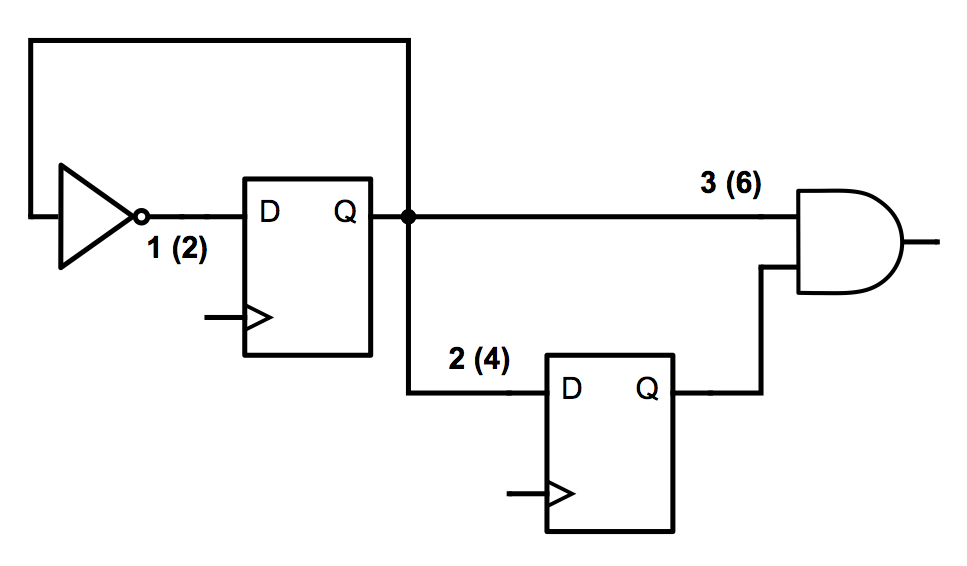
\includegraphics[width=100mm]{circuit.png}
\caption{The circuit represented in {\tt examples/simple3.aag}.}
\label{aagCircuit}
\end{figure}

For example, the circuit in Figure \ref{aagCircuit} is represented
as follows (comments to the right are not part of the specification):
\begin{lstlisting}[escapeinside = {*}{*}]
aag 3 0 2 1 1
2 3              *{\it D-latch (output wire has index 2)}*
4 2              *{\it D-latch (output wire has index 4)}*
6                *{\it Output}*
6 2 4            *{\it AND gate}*
\end{lstlisting}
The circuit has no inputs, two latches and one AND gate
whose output is the output of the whole circuit.
}


\section{MiniSat}
\label{prep:minisat}

This section provides some knowledge about MiniSat necessary
for creating an interface to MiniSat. The MiniSat code
explained is in C++.

To solve a SAT query, MiniSat creates an instance of a \verb,Solver, object,
which contains a set of variables, sets of clauses, and possibly a model or conflict vector.
The set of variables in the \verb,Solver, gives all the variables that may appear in
a SAT query, the set of clauses helps form the SAT query, and the model or conflict vector
gives further information about the last SAT query made.

Minisat represents variables with a \verb,Var, type and
literals with a \verb,Lit, type.
MiniSat represents sets of clauses as \verb,vec<Lit>,s,
vectors of literals. The conjunction of clauses in a \verb,Solver, represents a CNF query.
If the \verb,Solver,'s \verb,solve(), function is called,
the resulting \verb,bool, indicates the query's satisfiability.

The \verb,solve(), function is overloaded so that it may also take an assumption \verb,vec<Lit>*, as
an argument.
If the \verb,Solver,'s clauses form some CNF query $C$ and
\verb,solve(assumps), is called, where \verb,assumps, represents some set $A$ of literals,
then the SAT query is $C \wedge \bigwedge_{l \in A} l$.

If there has been at least one query made of the \verb,Solver, and the last query was
satisfiable, the \verb,Solver,'s \verb,model, variable points to a set of variable assignments
for that SAT query.
If there has been at least one query made of the \verb,Solver, and the last query was
unsatisfiable, the \verb,Solver,'s \verb,conflict, variable points to a set of literals that
contains the assumed literals that caused the query to be unsatisfiable.

\emph{MC} uses instances of \verb,SimpSolver,, a subclass of the \verb,Solver, class
that does simplification and returns full assignments, providing more useful results
for the queries that IC3 makes.

\section{The IC3 Algorithm}
\label{prep:ic3}
%Describe how the IC3 algorithm works when trying to prove a model has a property
%$P$.
This section describes the basic IC3 algorithm and some of its extensions.
Given a hardware model (i.e. a finite-state transition system $(i,x,I,T)$) and a
safety property $P$, IC3 aims either to prove inductively that $P$ holds
at all states reachable from the initial state or
to find a reachable $\neg P$ state.
The pseudocode in Figure \ref{overview} gives an overview of the basic IC3 algorithm.	

\begin{algorithm}[t]
\DontPrintSemicolon
\Fn{prove$((i,x,I,T),P)$}{
  \lIf{$\neg (I \Rightarrow P)$ \label{initiation}}{
    \Return{False}
  }
  $F_0 := I$ \;
  $k := 0$ \;
  \While{True \label{main}}{
    \eIf{$F_k \wedge T \Rightarrow P'$ \label{consecution}}
    {create frame $F_{k + 1}$ initialized to $\emptyset$ \label{create} \;
     $k$ := $k + 1$ \;}
    {\While {$\neg (F_k \wedge T \Rightarrow P')$ \label{reconsec}}{
        ${\it cti} := {\it nextCTI}(F_k \wedge T \Rightarrow P')$ \label{CTI} \;
        \lIf{{\it proveNegCTI}$((i,x,I,T),{\it cti},k - 1)$ \label{negCTI}}{$F_k$ := $F_k \cup \{\neg{\it cti}\}$}
        \lElse{\Return{False}}}} \label{Unsafe}
    \For{ i = 0 \KwTo $k - 1$ }{ \label{forprop}
      $F_{i + 1} := F_{i + 1} \cup \{c \in F_i | F_i \wedge T \Rightarrow c'\}$ \label{push} \;
      \lIf {$F_i = F_{i + 1}$}{\Return {True}} \label{fixed}
    }
  }
}
\caption{Overview of IC3. Frames are passed by reference.}
\label{overview}
\end{algorithm}

The IC3 algorithm maintains a set of $k + 1$ frames $F_0,\ldots,F_k$.
Each frame $F_i$ is a set of clauses whose conjunction represents an
over-approximation of the set of states reachable by the transition
system in at most $i$ steps from the initial state (e.g. $F_0 = I$).
The deepest frame $F_k$ in the set of frames is the \emph{frontier}.

%Initiation query
The \emph{initiation query} $I \Rightarrow P$ (line \ref{initiation}) checks that
the property $P$ holds in the initial state $I$.
%This query is run once at the start of
%the algorithm for the desired property.
If it fails (i.e. does not hold), then the algorithm terminates;
a state in which $\neg P$ holds is reachable in 0 steps.
If it succeeds, then the algorithm enters its main loop (line \ref{main}).

%The main loop of the algorithm is the while loop beginning on line \ref{main}.
The algorithm only exits its main loop when it has determined whether or not the
safety property holds at all reachable states in the model.

%Consecution query
The \emph{consecution query} $F_k \wedge T \Rightarrow P'$ (line \ref{consecution})
checks whether the property $P$ holds in the next
frame. If it does, then IC3 creates a new
frontier frame $F_{k + 1}$ (line \ref{create}).
%Describe what happens when a consecution query fails

If a consecution query $F_k \wedge T \Rightarrow P'$ fails, then
there is an $F_k$ state $s_k$ and a $\neg P'$ state $s_{k + 1}$ with $T(i,s_k,s_{k + 1})$.
The state $s_k$ is called a \emph{counterexample to induction} (CTI).
The algorithm then aims to refine the approximation $F_k$ of the set of states
reachable in at most $k$ steps by showing that all states that are
reachable in at most $k$ steps are $\neg s_k$ states.

The call to {\it nextCTI} (line \ref{CTI}) finds the CTI
state $s_k$. When passed parameters $s = s_k$ and $j = k$,
the call to {\it proveNegCTI} (line \ref{negCTI})
attempts to prove that $\neg s$ is inductive relative to $F_{k - 1}$,
in which case all $F_k$ states are necessarily $\neg s$ states, so $\neg s$ can
be added to the set of $F_k$ clauses.

%The {\it proveNegCTI} algorithm works similarly to the
%while loop on line \ref{reconsec}.
While the query
$F_k \wedge \neg s \wedge T \Rightarrow s'$ is unsuccessful,
the algorithm extracts a CTI and
calls {\it proveNegCTI} to show that the counterexample is
inductive relative to frame $F_{j - 1}$ so that the negated
counterexample can be added to frame $F_j$.
If the shallowest possible depth $j = 0$ is reached, then
{\it proveNegCTI} fails and returns {\it False}.

The {\it proveNegCTI} pseudocode in Figure \ref{proveNegCTI}
does not explicitly check for $I \Rightarrow
\neg s$ because if
$I \Rightarrow \neg s$ does not hold, then eventually ${\it proveNegCTI}$
will be called recursively with $j = 0$, and the attempt to show that
$\neg s$ is relatively inductive to $F_j$ will fail.

\begin{algorithm}[t]
\DontPrintSemicolon
\Fn{proveNegCTI$((i,x,I,T),s,j)$}{
  \lIf{$j = 0$}{\Return{False}}
  \While{$\neg(F_j \wedge \neg s \wedge T \Rightarrow \neg s')$}{
    ${\it cti} := {\it nextCTI}(F_j \wedge \neg s \wedge T \Rightarrow \neg s')$ \;
    \lIf{{\it proveNegCTI}$((i,x,I,T),{\rm cti},j - 1))$}{$F_j$ := $F_j \cup \{\neg{\it cti}\}$}
    \lElse{\Return{False}}
  }
}
\caption{Pseudocode for proving negated CTIs.}
\label{proveNegCTI}
\end{algorithm}

If $\neg s_k$ cannot be proven to hold at each of $k$ steps of
the transition relation from the initial state, i.e., $s_k$ is in the actual
set of states reachable in $k$ steps from the initial state, then a $\neg P$ state
is reachable in $k + 1$ steps from the initial state; the safety property does not
hold, and the algorithm terminates (line \ref{Unsafe}).

Because there may be several CTIs,
the consecution query must be performed again (line \ref{reconsec}). If it fails again,
the process of finding the new CTI $d$ and trying to
prove that $\neg d$ holds at depth $k$ repeats.
When the consecution query succeeds, the algorithm moves to the propagation phase.

\emph{Pushing} a clause $c$ from frame $F_i$ to frame $F_{i + 1}$ refers to the act
of setting $F_{i + 1} := F_{i + 1} \cup \{ c \}$ with $c \in F_i$.
A clause $c$ can be pushed from frame $F_i$ to the next frame $F_{i + 1}$
if the consecution query $F_i \wedge T \Rightarrow c'$ holds.
The propagation phase of the algorithm goes through the set of frames
$F_0, \ldots, F_k$, and, for every $F_i$ with $0 \leq i < k$ (line \ref{forprop}),
pushes all the clauses that it can from $F_i$ to $F_{i + 1}$ (line \ref{push}).

If $F_i = F_{i + 1}$ holds for any $i$ at any point, then a fixed point has
been found; all the clauses in $F_i$ and therefore $F_{i + 1}$
can be pushed.
Because $F_i$ contains the safety property $P$ as one of its clauses,
$P$ holds in all reachable states from the initial state,
and the algorithm terminates (line \ref{fixed}). Because the number of
clauses in each frame $F_i$ decreases monotonically as $i$ increases and the
frame $F_0$ can only have finitely many states, the algorithm always
terminates.

\subsection{Inductive Generalization}

After showing that a negated CTI state $\neg s$ is relatively inductive to a
frame $F_i$ and adding the clause $\neg s$ to frame $F_{i + 1}$, the state
$s$ is eliminated from $F_{i + 1}$. An improvement can be made by generalizing
the single state $s$ to a set of several states $c$ and treating
$c$ as the CTI. If $\neg c$ is successfully proven to be relatively inductive
to $F_i$, then adding it to frame $F_{i + 1}$ eliminates several states (i.e.,
all $c$ states) at once rather than only $s$. Because the cube $c$
is chosen so that $\neg c \Rightarrow \neg s$, at least one CTI state
has been removed from $F_{i + 1}$, and because $c$ contains several states,
it is possible that several CTIs may have been removed from $F_{i + 1}$
by adding the clause $\neg c$ to it. The process of finding such a cube $c$
is referred to as \emph{generalization}, and the best such $c$ is the
one such the $\neg c$ is the minimal inductive subclause for $F_i$ and $\neg s$.

\subsection{Minimal Inductive Subclauses}
The \emph{minimal inductive subclause} (MIC) for a frame $F_i$ and a clause $\neg s$
inductive relative to $F_i$
is the smallest subclause $\neg c$ of $\neg s$ s such that
$\neg c$ is also inductive relative to $F_i$.
The MIC can be found by dropping each literal
in $\neg s$ in turn and checking the resulting clause.

The checking phase (described by {\it down} in Figure \ref{mic},
which takes a clause ${\it cls} = \neg s$ and a depth $i$ as arguments)
performs queries
for determining whether the subclause is inductive relative to
$F_i$: for a subclause $t = \neg s \setminus \{l\}$ obtained by dropping
literal $l$ from $\neg s$, it checks that
$I \Rightarrow t$ and $F_i \wedge t \wedge T \Rightarrow t'$ both hold.

If both formulas hold, then $l$ can be dropped from $\neg s$.
If only $F_i \wedge t \wedge T \Rightarrow t'$ fails to hold, then
expanding the set of states in $t$ by removing %some of the
literals in $t$ could result in a clause that is inductive relative to $F_i$.
If $I \Rightarrow t$ fails to hold, then removing literals in $t$ to
obtain a subclause $u \subset t$ would still result in the query $I \Rightarrow u$
failing, since $u \Rightarrow t$ holds.

If $F_i \wedge t \wedge T \Rightarrow t'$ does not hold, then
there is a predecessor to a $\neg t$ state that is a $F_i \wedge t$ state.
This predecessor state $p$ can be extracted from the SAT query for
$F_i \wedge t \wedge T \Rightarrow t'$ in the same way that CTIs are found.
The clause $t$ can then be expanded to the clause $t \cap \neg p$
formed by taking the common literals in $t$ and $\neg p$.
The checking phase then repeats, checking the expanded clause $t \cap \neg p$.

\begin{algorithm}[t]
\DontPrintSemicolon
\Fn{mic(cls,i)}{
  \ForEach{literal l in cls}{
    $subcls := cls \setminus \{l\} $\;
    \If{${\it down(subcls, i)}$}{
      $cls := subcls$ \;
    }
  }
  \Return{cls} \;
}
\Fn{down(cls, i)}{
  \lIf{$\neg (I \Rightarrow {\it cls})$}{\Return{False}}
  \lIf{$F_i \wedge {\it cls} \wedge T \Rightarrow {\it cls}'$}{\Return{True}}
  $p$ := $F_i \wedge t$ state such that $F_i \wedge t \wedge p \Rightarrow \neg t'$ \;
  {\it cls} := $cls \cap p$\;
  \Return{down(cls,i)} 
}
\caption{Algorithm for finding the MIC. Clauses are
passed by reference.}
\label{mic}
\end{algorithm}

Considering counterexamples to generalization can result in more effective
generalization \cite{hassan13}.

\subsubsection{Counterexamples to Generalization}

For a subclause $\neg c = s \setminus \{l\}$ of a clause $\neg s$ to be
inductive relative to a frame $F_i$, the implication
$F_i \wedge T \wedge \neg c \Rightarrow \neg c'$ must hold.
In the method of generalization described above,
if it does not hold,
$\neg s$ cannot be generalized to $\neg c$, and generalization
proceeds without dropping $l$.

Similarly to why a consecution query at $F_k$ may fail,
$F_k \wedge T \wedge c \Rightarrow c'$ might be unsatisfiable because
$F_k$ is too loose an approximation. As with consecution queries, discovering a
new clause that can be added to $F_k$ may allow queries that
check for relative induction to succeed. The discovery of this
clause can be directed by a counterexample extracted from the
SAT solver after the query for $F_k \wedge T \wedge c \Rightarrow c'$.

This counterexample is called a \emph{counterexample
to generalization} (CTG), and proving the negated CTG to be true at
frame $F_k$ allows $s$ to be generalized to $c$.


\chapter{Implementation}
\label{impl}

\begin{figure}[t]
\tikzstyle{io}=[fill=white,scale=0.8]
\tikzstyle{component}=[rectangle,draw,fill=white,scale=0.9]
\tikzstyle{label}=[font=\footnotesize]
\begin{tikzpicture}[auto, scale = 0.6]
  \node (input) [io] {AIGER Input};
  \node (parser) [component, below of=input] {Parser}
    edge [<-] (input);
  \node (representation) [component, right=1em of parser]
    {Conversion to Appropriate Representation}
    edge [<-] (parser);
  \node (mc) [component, right=1em of representation]
    {Model Checker}
    edge [<-] (representation);
  \node (iminisat) [component, right=1em of mc]
    {MiniSat Interface}
    edge [<->] (mc);
  \node (minisat) [io, above of=iminisat]
    {MiniSat}
    edge [<->] (iminisat);
  \node (output) [io, above of=mc] {Output}
    edge [<-] (mc);
\end{tikzpicture}
\caption{Interaction among main components.}
\label{components}
\end{figure}

This chapter describes the implementation of \emph{MC}.
The implementation can be broken up into four main components
(see Figure \ref{components}): the AIGER parser
(Section \ref{impl:aiger}), the
MiniSat interface (Section \ref{impl:minisat}), the hardware model representation
(Section \ref{impl:representation}), and the back end
(Section \ref{impl:modelchecker}).
The implementation of the AIGER parser, MiniSat interface, and \emph{Basic} version
of the IC3 algorithm satisfy the project aims to implement these components. As
extensions, I have implemented additional variants of the IC3 algorithm in different
versions of the back end.

The variants of the back-end component differ
in their overall structure,
finding of CTIs, implementations of propagation, and
inductive generalization of CTIs. The following table
summarizes the variants and their
differences:\\

\begin{tabular}{| l | p{3.5em} | p{3em} | p{4.5em} | p{5em} | p{6em} |}
\hline
& Priority Queue & Smaller CTIs & Subsumed Clauses & Basic Generalization & Generalization with CTGs\\
\hline
\emph{Basic} & & & & \checkmark & \\
\emph{BetterCTI} & & \checkmark & & \checkmark & \\
\emph{BetterPropagation} & & \checkmark & \checkmark & \checkmark &\\
\emph{PriorityQueue} & \checkmark & \checkmark & \checkmark & \checkmark & \\
\emph{CTG} & & \checkmark & \checkmark & & \checkmark \\
\hline
\end{tabular}\\



%I now briefly explain the motivations for the deviations from the \emph{Basic}
%implementation. The details of these deviations are given in Section \ref{impl:modelchecker}.
The ``Priority Queue'' alteration was based on the observation that implementations
using priority queues tend to be more efficient than simple
recursive implementations of the IC3 algorithm \cite{een11,griggio14}.
The ``Smaller CTIs'' alteration was based on the improvement of finding
predecessors to counterexamples that describe sets of several states rather
than singleton states \cite{griggio14}.
The ``Subsumed Clauses'' alteration was based on the observation that subsumed clauses slow
down the SAT-solver and should be eliminated to achieve better performance
\cite{een11}.
The ``Generalization with CTGs'' alteration was based on the description of an algorithm
that improves upon basic inductive generalization \cite{hassan13}.

\section{Parser}
\label{impl:aiger}
%Discuss the implementation of the AIGER parser. In particular, mention
%the handling of both the older and newer AIGER format versions for both
%the ASCII and binary versions of the format and the representation
%of AIG models.

%The relevant files for this section can be found in the \verb,Parser, directory.
The parser component parses ASCII or binary-formatted AIGER files and
assumes that the new format is used
(note that the new format is backward compatible).
Justice properties and fairness constraints are not handled by \emph{MC}, so
the parser ignores them.

The \verb,Parser.AigerParser, module, which implements the parser in Haskell, and
the \verb,Parser.AigerTools, module, which calls the Aiger Utilities' parser's functions,
each convert the AIGER file into the \verb,Model, data structure in \verb,Parser.AigModel,,
which stores the components specified in the AIGER file.

\subsection{Model}

The \verb,Model, data structure stores the number of variables and
inputs as well as lists of literals that represent outputs, bad states,
and invariant constraints. It also stores latches and AND gates as
lists of literal lists. Below, I discuss the representation of literals, latches, and
AND gates.

Literals are represented by \verb,Lit,s (defined in Section \ref{prep:haskell}),
which store decoded versions of AIGER indices. The {\tt Lit} datatype
in {\tt Parser.AigModel} has the following constructors:
\begin{itemize}
\item \verb,Boolean,, which takes a \verb,Bool, argument;
\item \verb,Var,, which takes a \verb,Word, argument; and
\item \verb,Neg,, which takes a \verb,Word, argument.
\end{itemize}
\verb,Boolean,s represent the Boolean values corresponding to AIGER indices 0 and 1,
and \verb,Var, and \verb,Neg, respectively represent the positive or negative literal
of the variable whose name is given by the \verb,Word, the constructor takes as an
argument.
Variable names are adjusted (by subtracting 1) so that they start at 0.
For example, the AIGER index 3 is parsed to \verb,Neg 0,;
the odd index 3 specifies a negative literal of the variable 1;
subtracting by 1 gives the new variable name 0.

Latches and AND gates are represented by three-element \verb,[Lit],s. For latches,
\begin{itemize}
\item the first element gives the latch's output (i.e. variable name)
as a positive literal,
\item the second gives the latch's input (i.e. the next-state literal), and
\item the final element gives the latch's initial state.
\end{itemize}
For example, the latch from Figure \ref{aagCircuit} represented by \verb,2 3, is parsed
to \verb.[Var 0, Neg 0, Boolean False]..

For AND gates,
\begin{itemize}
\item the first element gives the AND gate's output (i.e. variable name)
(as a positive literal), and
\item the next two elements give the literals whose values are the AND gate's inputs.
\end{itemize}
For example, the AND gate from Figure \ref{aagCircuit} represented by \verb,6 2 4, is
parsed to \verb.[Var 2, Var 0, Var 1]..

The full AIGER representation for the circuit in Figure \ref{aagCircuit} is
as follows:
\begin{lstlisting}
Model { numVars = 3
      , numInputs = 0
      , latches = [ [Var 0, Neg 0, Boolean False]
                  , [Var 1, Var 0, Boolean False] ]
      , outputs = [Var 2]
      , ands = [ [Var 2,Var 0,Var 1] ]
      , bad = []
      , constraints = []}
\end{lstlisting}

\section{MiniSat Interface}
\label{impl:minisat}
%Describe the process of implementing the Haskell bindings for Minisat
%functions, including the wrapper functions for Minisat written in C.

\emph{MC} uses the MiniSat SAT solver.
Because the Haskell Foreign Function Interface (FFI) cannot interface with C++ directly,
the interface to the MiniSat SAT solver is composed of a C wrapper for relevant
MiniSat functions and classes and a Haskell interface to the C wrapper.

The C wrapper replaces each MiniSat class with a C type and each MiniSat function with
an \verb,extern C, function that calls the MiniSat C++ function.
For instance, the following function
in \verb,Minisat/CSolver.cpp, is a wrapper for \verb,addClause, in the \verb,Solver,
class:
\begin{lstlisting}[language = C++]
extern "C" int addMinisatClause (Minisat::SimpSolver* solver,
                                 Minisat::vec<Minisat::Lit>* ps) {
  return solver -> addClause (*ps);
}
\end{lstlisting}

The FFI is then used to provide a wrapper function that calls
the C function:
\begin{lstlisting}
foreign import ccall safe "addMinisatClause"
  addMinisatClause :: Ptr MinisatSolver -> Ptr MinisatVecLit -> IO CInt
\end{lstlisting}

Just using the FFI to call C functions does not provide a
sufficient abstraction for an interface used by the rest of \emph{MC}. All
calls to C functions must occur inside the \verb,IO, monad, but having
the interface functions return \verb,IO, monads means that any functions
using interface functions to get values from MiniSat would also need to
perform all their computations inside the \verb,IO, monad, requiring them to
be written imperatively.
Additional functions use a Haskell idiom for providing a more natural
interface for C libraries; they use \verb,unsafePerformIO, to return
values outside the \verb,IO, monad.

The \verb,solveWithAssumps, function can be called to
solve a query with MiniSat (see Figure \ref{solveWithAssumps}),
taking a solver \verb,s, and a list of literals \verb,assumps,
that make up the assumption vector. The \verb,solveWithAssumps, function
visible to other modules uses Haskell wrapper functions to create
a MiniSat \verb,vec<Lit>, to represent the assumption vector and call
the C wrapper function \verb,solveMiniSatWithAssumps,.

The function \verb,solveMinisatWithAssumps,, a wrapper for the version of \verb,solve(),
that takes an assumption vector as an argument, returns a pointer to a
\verb,result, struct instead of, like the MiniSat \verb,solve(), function,
just an indication of the query's satisfiability.
The Haskell interface uses the FFI and \verb,hsc2hs, preprocessor
for handling the \verb,result, struct. For example, \verb,solveWithAssumps,
uses the FFI's \verb,peek, function,
which provides a value read from a memory location inside
an \verb,IO, monad, to read in the \verb,result, struct. After unmarshalling
the \verb,result, struct into a Haskell \verb,Result, datatype, \verb,solveWithAssumps,
uses \verb,unsafePerformIO, to extract the \verb,Result, from the \verb,IO, monad.

The \verb,result, struct in \verb,Minisat/CSolver.h,
allows a single function call to return
all the information from solving a SAT query. The struct contains an indication of query satisfiability
and pointers to the model and conflict vector (if any) of the \verb,Solver,:
\begin{lstlisting}[language=C]
struct result {
  unsigned solved;
  unsigned modelSize;
  unsigned conflictSize;
  minisatLbool* model;
  litptr* conflict;
} res = {0, 0, 0, 0, 0};
\end{lstlisting}

\begin{figure}[t]
\centering
\tikzstyle{io}=[font=\small\tt, scale=0.7]
\tikzstyle{function}=[rectangle,draw,minimum width=4em,fill=white,font=\small\tt,scale=0.8]
\begin{tikzpicture}[auto, scale = 0.6]
  \node (call) [io] {};
  \node (haskell) [function, right = 7em of call]
    {solveWithAssumps s assumps {\it (Haskell MiniSat Interface)}}
    edge [<-] (call);
  \node (haskellffi) [function, below = 1.5em of haskell]
    {solveMinisatWithAssumps sol veclit {\it (Haskell FFI)}}
    edge [<-, bend left] (haskell);
  \node (wrapper) [function, below = 1.5em of haskellffi]
    {solveMinisatWithAssumps (solver, assumps)
      {\it (C wrapper)}}
    edge [<-, bend left] (haskellffi);
  \node (minisat) [function, below = 1.5em of wrapper]
    {solver -> solve(*assumps) {\it (MiniSat)}}
    edge [<-, bend left] (wrapper);
  \node (ret) [io, right = 7em of haskell] {};
  \draw [->, bend right] (minisat) to node [swap,io] {solved} (wrapper);
  \draw [->, bend right] (wrapper) to node [swap,io] {\&res} (haskellffi);
  \draw [->, bend right] (haskellffi) to node [swap,io] {peek} (haskell);
  \draw [->] (haskell) to node [io] {unsafePerformIO res} (ret);
\end{tikzpicture}
\caption{Function calls for {\tt solveWithAssumps}.}
\label{solveWithAssumps}
\end{figure}

The information kept in a \verb,Result, Haskell datatype comes directly from the
\verb,result, returned by the C wrapper functions.
I used \verb,hsc2hs, to handle pointer offsets
when unmarshalling from the C struct.
Beyond straightforward unmarshalling, some additional work was necessary
to convert from the MiniSat representation of literals to the \emph{MC} representation.

MiniSat variable $2 \times x$ represents the variable with name $x$, where $x$ is a nonnegative
integer; MiniSat variable $(2 \times x) + 1$ represents
$x'$.
The \verb,model, returned in the \verb,result, struct
points to an array of three-valued Boolean (the normal Boolean values and an
\emph{undefined} value) \verb,lbool, values indexed by MiniSat variable indices.
To extract models, the array values are accessed; for each \emph{True} or \emph{False}
value the positive or negative literal for that index is added to the
\verb,[Lit], representing the model.

\section{Hardware Representation}
\label{impl:representation}
This section describes the representation and construction of hardware models (i.e.
transition systems) and frames in \emph{MC}.

\subsection{Model Representation}
\subsubsection{Literals and Clauses}
The \verb,Lit, data structure in \verb,Model.Model, represents literals in
the back end.
The \verb,Var, and \verb,Neg, constructors respectively give positive and negative
current-state (unprimed) literals, and the \verb,Var', and \verb,Neg', constructors
respectively give positive and negative next-state (primed) literals.
A clause is represented with type \verb,Clause,, where each \verb,Clause, is a
list of the \verb,Lit,s in the clause.

\subsubsection{Transition Systems and Safety Properties}
% Describe how transition systems and safety properties are represented.
The \verb,Model, data structure in \verb,Model.Model, encompasses both
the representation of transition systems and the safety property for the back end to check.
It represents the hardware in the back end:
\begin{lstlisting}
data Model = Model { vars :: Word
                   , initial :: [Clause]
                   , transition :: [Clause]
                   , safe :: Lit } deriving Show
\end{lstlisting}

Inputs $i$ and state variables $x$ in the transition system $T(i,x,I,T)$
are not distinguished; both are just represented as variables.
The total count of variables is kept in \verb,vars,.
Clauses that specify the initial state $I$ are kept in \verb,initial,.
The \verb,transition, list of clauses that specify latches and AND
gates capture the transition relation $T$.
The \verb,safe, literal gives the safety property.

\subsection{Model Construction}
% Describe how transition systems are constructed given AIG models.

The \verb,Model.Model, module contains functions to convert the \verb,Model, data
structure from the \verb,Parser.AigModel, module into the model representation
used by the back end. In particular, \verb,toModel, takes a \verb,Parser.AigModel.Model,
and outputs a \verb,Model.Model.Model,. The \verb,Model.Model.Lit,
data structure only has constructors for variables and their negations,
with the following datatype declaration:
\begin{lstlisting}
data Lit = Var Word | Neg Word | Var' Word | Neg' Word deriving (Show, Eq, Ord)
\end{lstlisting}
All \verb,Lit,s from
the \verb,Parser.AigModel, module are either converted to \verb,Model.Model.Lit,s or, if
they use the \verb,Boolean, constructor, are removed from the model during the conversion of
the \verb,Latch, and \verb,And, components to \verb,Clause,s in \verb,Model.Model,.
%because Boolean values are not used in these representations.

\subsubsection{Latches}
The \verb,makeLatches, function generates a pair of \verb,Clause, lists
for a list of \verb,Parser.AigModel.Latch,es. The first list contains
clauses whose conjunction describes the latches' initial values,
and the second contains a clauses whose conjunction describes the
latches' next-state values.

Consider a given \verb,Parser.AigModel.Latch, $[l, n, i]$ representing the latch with
output $l$, next state $n$, %taken from the set of literals,
and initial value $i$.
%also taken from the set literals.
The \verb,makeLatches, function uses the
values of $l$, $n$, and $i$ to generate \verb,Clause,s that describe the latches' initial values and
next-state values.

Generating the initial value clause of the latch proceeds as follows: if $i = {\it True}$,
then the singleton clause $\{l\}$ is generated for the initial value list, and if $i = {\it False}$,
then the singleton clause $\{\neg l\}$ is generated.
If $i$ is a literal rather than a Boolean value, then the latch is
uninitialized and no clauses are generated for its initial value.

Generating next-state clauses proceeds similarly.
By the semantics of latches, the generated next-state clauses should have
a conjunction logically equivalent to $n \Leftrightarrow l'$.
If $n = {\it True}$, then singleton clause
$\{l'\}$ is generated because the next-state value for the variable is a constant-{\it True} value,
and if $n = {\it False}$, then singleton clause $\{\neg l'\}$ is generated.
Otherwise, if $n$ is not a Boolean value,
the next-value clauses generated for $l$, are $\{l', \neg n\}$
and $\{\neg l', n\}$. The conjunction of these clauses are, as needed, logically equivalent
to $n \Leftrightarrow l'$, i.e., where $\simeq$ denotes logical equivalence,
$$l' \Leftrightarrow n \simeq (\neg l' \vee n) \wedge (l' \vee \neg n).$$

\subsubsection{AND gates}
The \verb,makeAnds, function generates a single \verb,Clause, list for a list of \verb,Parser.AigModel.And,s,
where the conjunction of the clauses in the list describes the relationship between the AND-gate's output
and inputs.

Consider a \verb,Parser.AigModel.And, of the form $[a, i_1, i_2]$ representing the AND gate
with output $a$ and inputs $i_1$ and $i_2$.
The \verb,makeAnds, function uses the values of $a$, $i_1$, and $i_2$ to generate
\verb,Clause,s that describe the AND gate.
By the semantics of AND gates, the generated current-state clauses should have a conjunction
logically equivalent to $a \Leftrightarrow (i_1 \wedge i_2)$ and the generated next-state
clauses should have a conjunction logically equivalent to
$a' \Leftrightarrow i_1' \wedge i_2'$. The next-state clauses are generated
by priming the generated current-state clauses, so they satisfy
$a' \Leftrightarrow i_1' \wedge i_2'$.

If both inputs are Booleans (i.e. both use \verb,Parser.AigModel.Lit,'s \verb,Boolean,
constructor), then a singleton clause sufficiently describes the AND gate.
If $i_1 \wedge i_2$ holds, then $\{a\}$ describes this constantly {\it True} AND gate.
If not, then $\{\neg a\}$ describes this constantly {\it False} AND gate.

If only one input is a Boolean, then if it is {\it False},
singleton clause $\{\neg a\}$ is generated. If it is {\it True},
the clauses equivalent to $a \Leftrightarrow i$ (i.e.
$\{i, \neg a\}$ and $\{\neg i, a\}$)
are generated, where $i$ is the input that is not a Boolean.

If neither $i_1$ nor $i_2$ are Booleans, then \verb,makeAnds, generates
$\{\neg a, i_1\}$, $\{\neg a, i_2\}$, and
$\{\neg i_1,\neg i_2, a\}$. The conjunction of these clauses are, as needed,
logically equivalent to $a \Leftrightarrow (i_1 \wedge i_2)$:
$$a \Leftrightarrow (i_1 \wedge i_2) \simeq
(\neg a \vee i_1) \wedge (\neg a \vee i_2) \wedge (\neg i_1 \vee \neg i_2 \vee a).$$

\subsection{Frames}
In addition to a representation of transition systems, \emph{MC} needs a representation
of the frames used by the IC3 algorithm.
The \verb,Frame, data structure represents frames in all back ends.
Along with the set of clauses (represented by a list of literals), a \verb,Frame, also
includes a \verb,Solver,, which contains at least all the clauses in the frame's set
of clauses.
The \verb,Solver, may also contain the \verb,transition, clauses for the hardware model.

\section{Model Checking}
\label{impl:modelchecker}

I implemented several variants of the IC3 algorithm:
\emph{Basic}; \emph{BetterCTI}, which improves upon \emph{Basic} by discovering
smaller CTIs; and \emph{BetterPropagation}, which improves upon \emph{BetterCTI}
by considering subsumed clauses
I also implemented a variant that uses priority queues (\emph{PriorityQueue})
and a variant that uses CTGs to improve generalization (\emph{CTG}).

I describe the overall structure shared by all variants except
\emph{PriorityQueue} before describing the implementation
details of smaller components of the algorithm and how they differ across
variants. A separate description of \emph{PriorityQueue}
follows.

\subsection{Overall structure}

The structure of the algorithm in the implementations is similar
to Figure \ref{overview}; however, there are
small differences that result from implementing the algorithm in a
functional language and adjusting how the propagation phase is
carried out.

The pseudocode in Figure \ref{recstr}
outlines the structure shared by all the \emph{MC}
implementations except {\it PriorityQueue}.
I compare this structure with Figure \ref{overview} (see Section
\ref{pqueue} for \emph{PriorityQueue}).
The main components of the algorithm in Figure \ref{recstr} are as follows:
\begin{itemize}
\item The {\it prove} component (line \ref{recstr:prove})
takes a model $M$ and a property $P$ as input
 and provides the same output as the \emph{prove} component in Figure \ref{overview}.
\item The ${\it prove'}$ component (line \ref{recstr:prove'})
takes a model $M$, a property $P$,
the frontier frame $F_k$, and the rest of the frames $[F_0,\ldots,F_k]$ as input. It
implements the main loop in Figure \ref{overview}, achieving the looping behavior with
recursive calls (lines \ref{recstr:recursion}, \ref{recstr:mutrecursion}).
\item The {\it pushFrame} component (line \ref{recstr:pushFrame}) takes the old frontier frame
$F_{k - 1}$ to push clauses from, the new frontier frame $F_k$ to push clauses to,
the model $M$, and the rest of the frames $[F_0, \ldots, F_k]$ as input.
It implements a specialized part of the propagation phase.
\item The {\it nextCTI} component (line \ref{recstr:nextCTI})
takes a failing consecution query as input and returns
a CTI, just as in Figure \ref{overview}.
\item The {\it proveNegCTI} component (line \ref{recstr:proveNegCTI})
takes a model $M$, a CTI, and a depth $k - 1$ as input and
returns a triple $({\it result}, [G_0, \ldots, G_{k - 1}], G_k)$, where {\it result}
is {\it False} iff the while loop containing {\it proveNegCTI} in Figure \ref{overview}
would return {\it False}.
Each $G_i$ gives the value that frame $F_i$ would have after the termination of
the while loop in Figure \ref{overview}.
\item The {\it propagate} component (line \ref{recstr:propagate})
takes the current frames $[G_0, \ldots, G_k]$ as input and
returns a pair $({\it fixed}, [H_0, \ldots, H_{k-1}, H_k])$, where {\it fixed} is {\it True}
iff the propagation phase loop in Figure \ref{overview} would have returned {\it True}.
Each $H_i$ gives the value that the frame $F_i$ would have after the propagation
phase updated it in Figure \ref{overview}. The Haskell implementation of this component
returns a \verb,Maybe [Frame],, where the function returns \verb,Nothing,
when {\it fixed} is {\it True}.
\item The {\it push} component (line \ref{recstr:push})
takes two frames $F$ and $F'$ as input and returns a
pair $({\it fixed}, G')$, where {\it fixed} is {\it True} iff all clauses in $F$ can
be pushed to $F'$ and $G'$ is the updated value of $F'$ after having pushed all possible
clauses from $F$ to $F'$.
\end{itemize}

\SetKwProg{Let}{let }{ in}{end}
\begin{algorithm}[t]
\DontPrintSemicolon
\Fn{prove$(M,P)$}{ \label{recstr:prove}
  \lIf{$\neg (I \Rightarrow P)$}{ \label{recstr:init}
    \Return{False}
  }
  \Return ${\it prove'}(M,P,I,{\rm nil})$ \label{recstr:prove'call}
}
\Fn{${\it prove'}(M,P,F_k,[F_0,\ldots,F_{k - 1}])$ \label{recstr:prove'}}{
  \eIf{$F_k \wedge T \Rightarrow P'$ \label{recstr:consecution}}
  {\Return{{\it pushFrame}$(F_k, \emptyset,M,P,[F_0,\ldots,F_{k - 1}])$} \label{recstr:pushFrameCall}}
  {\Let{{\it cti} = {\it nextCTI}$(F_k \wedge T \Rightarrow P')$ \label{recstr:nextCTI}, \;
  $({\it result}, [G_0,\ldots,G_{k - 1}], G_k)$ = {\it proveNegCTI}$(M,{\rm cti},k - 1)$ \label{recstr:proveNegCTI}} 
  {
  \If{\it result} {
    \Let{$({\it fixed}, [H_0,\ldots,H_{k - 1},H_k]) = {\it propagate}([G_0,\ldots,G_{k - 1},G_k])$}{ \label{recstr:propagate}
    \lIf{\it fixed}{\Return{True}}
    \lElse{\Return{${prove'}(M,P,H_k,[H_0,\ldots,H_{k - 1}])$} \label{recstr:recursion}}}}
  \lElse{\Return{False}}}}
}
\Fn{pushFrame$(F_{k - 1}, F_k,M,[F_0,\ldots,F_{k - 2}])$}{ \label{recstr:pushFrame}
  \Let{$({\it fixed}, G_k) = {\it push}(F_{k - 1}, F_k)$ \label{recstr:push}}{
  \lIf{\it fixed}{\Return{True}}
  \lElse{\Return{${\it prove'}(M, P, G_k, [F_0,\ldots,F_{k - 2},F_{k - 1}])$} \label{recstr:mutrecursion}}}
}
\caption{General structure of most \emph{MC} back ends. The transition relation $T$ is acquired
from model $M$.}
\label{recstr}
\end{algorithm}

Because the implementation \emph{MC} is in Haskell, the
structure of the algorithm has been modified to be recursive rather than iterative.
The {\it prove} function (line \ref{recstr:prove}) makes an initiation query
(line \ref{recstr:init}), and, if it succeeds, calls
{\it prove'} (line \ref{recstr:prove'call}),
which corresponds to a recursive version of the main while loop
in line \ref{main} of Figure \ref{overview}.

Because Haskell functions are pure, the assumption made in Figure \ref{overview}
that functions can modify the set of (passed-by-reference) frames can no longer be made.
Instead, updated values of frames are returned explicitly by the function in
a tuple along with any other values needed from the function call, as seen in
{\it proveNegCTI}, {\it propagate}, and {\it push}.

In addition to making necessary language-related modifications to the algorithm, I 
reduced how often the full propagation phase executes, calling {\it pushFrame}
(line \ref{recstr:pushFrame}) instead where appropriate.

If the consecution query (line \ref{recstr:consecution}) succeeds, then
considering pairs of frames other
than $(F_{k - 1}, F_k)$, where $F_{k - 1}$ is the old frontier frame and $F_k$ is
the newly-created frontier frame, is unnecessary work.
Since no frames have been updated, there is nothing to push to frames $F_i$ with
$0 \leq i < k$.
The modified algorithm is such
that when the consecution query succeeds, it calls the ${\it pushFrame}$ function
(line \ref{recstr:pushFrameCall}) that
checks only a single pair of frames (and also makes the recursive call to ${\it prove}$).
When the consecution query fails, the adjusted algorithm, like the original in Figure \ref{overview},
calls ${\it propagate}$ (line \ref{recstr:propagate})
to handle the updates to the frames made by ${\it proveNegCTI}$.

\subsection{Initiation}
%Describe how the step involving the initiation query is implemented.

The initiation query $I \Rightarrow P$ is an implication, but a MiniSat \verb,Solver, can only
solve CNF queries (with an optional assumption cube).
As a result, all variants use the fact that
$I \Rightarrow P$ holds iff $\neg P \wedge I$ is unsatisfiable to yield
the following implementation in \verb,IC3.hs,:

\begin{lstlisting}
initiation :: Frame -> Clause -> Bool
initiation f prop =
  not (satisfiable (solveWithAssumps (solver f) (map neg prop)))
\end{lstlisting}

\subsection{Consecution}
%Describe how the step involving the consecution query is implemented.

Like the initiation query, the consecution query must be expressed in CNF.
All variants use the fact that
$F_k \wedge T \Rightarrow P'$ holds iff $\neg P' \wedge F_k \wedge T$ is unsatisfiable
to yield the following implementation:
\begin{lstlisting}
consecution :: Frame -> Clause -> Bool
consecution f prop =
  not (satisfiable (solveWithAssumps (solver f) (map (prime.neg) prop)))
\end{lstlisting}

\subsection{Counterexamples to Induction}
%Describe how the implementation discovers counterexamples
%to induction and proves them unreachable.

The \verb,nextCTI, function finds CTIs by
using results from SAT queries to find a full or partial assignment to
the variables in the \verb,Model,.

\subsubsection{Basic}
In \emph{Basic}, \verb,nextCTI, asks for a model
(i.e. the set of true literals) for the satisfiable query $\neg P' \wedge F_k \wedge T$.
The model's current-state literals then give a predecessor state (a state from which
a $\neg P$ state can be reached in one step of the transition relation) for $\neg P$,
i.e., the current-state literals give the CTI.
The function that called \verb,nextCTI, extracts these current-state literals from the model.

\subsubsection{Smaller Counterexamples to Induction}
In all implementations of the algorithm other than {\it Basic},
\verb,nextCTI, again asks for a model $m$
for the satisfiable query $\neg P' \wedge F_k \wedge T$. The only literals in $m$ that
must be included in the CTI are those current-state literals that result in
the unsatisfiability of $m \wedge P' \wedge T$. That is, the current-state literals of any
subcube $q$ of $m$ for which $q \wedge P' \wedge T$ holds is also a valid CTI, with
the state $m$ being in the set represented by $q$.

The conflict vector obtained from SAT-solver query $P' \wedge T$ and assumption
cube $m$ contains such a $q$ that has only literals relevant to the conflict. This $q$ is
then returned to the calling function, which, as in \emph{Basic}, extracts
the current-state literals from $q$ to obtain the CTI.


\subsection{Propagation}
\label{impl:propagation}
The implementations of both the {\it pushFrame} and {\it propagate} functions
in Figure \ref{recstr} (lines \ref{recstr:pushFrame},
\ref{recstr:propagate}) and
Figure \ref{pqueuestr} (lines \ref{pqueuestr:pushFrame}, \ref{pqueuestr:propagate})
rely on the implementation of the
{\it push} function, which has two variants described below.

\subsubsection{Basic}
The {\it Basic} and {\it BetterCTI} implementations' \verb,push, function,
when invoked as \verb,push f model f', tries to push all clauses in \verb,Frame, \verb,f,
that are not in \verb,Frame, \verb,f', to \verb,f', and
results in a pair containing a \verb,Bool, indicating whether a fixed point has been reached
(i.e., all clauses could be pushed) and a \verb,Frame, with all the clauses in \verb,f', and all
the clauses in \verb,f, that could be pushed to \verb,f',.
For each clause in \verb,f, that is not in \verb,f',, the \verb,consecution, function is called to
see if the clause is inductive relative to the frame \verb,f,. If it is, then
the clause can be added to \verb,f',, and if not, the
function must have \verb,False, as the first element in the pair it returns.

\subsubsection{Subsumed clauses}
The \emph{Basic} and \emph{BetterCTI} implementations' \verb,push, function avoids unnecessary
consecution queries by only considering clauses in \verb,f, that are not in \verb,f',.
Further consecution queries may be eliminated by removing subsumed clauses in \verb,f,,
which is done by all variants other than {\it Basic}
and \emph{BetterCTI}.

A clause $c$ \emph{subsumes} a clause $c'$ if $c$ is a subclause of
$c'$. In this case, $c \Rightarrow c'$ holds, so $c'$ can be removed from the set of clauses. By
removing subsumed clauses from a frame before trying to push clauses, \emph{MC}
can avoid making the consecution queries that arise from attempts to push those clauses.

Versions of \verb,push, that consider subsumed clauses include a call to the function
\verb,removeSubsumed, when acquiring the list of clauses to attempt to push.
The \verb,removeSubsumed, function takes a list of clauses and removes all clauses that are
subsumed by other clauses in the list.
The \verb,push, function replaces the frame
\verb,f, with a version of \verb,f, without subsumed clauses
for the rest of the function and proceeds as the basic implementation's \verb,push, function does,
returning a triple containing the updated \verb,f, along with the fixed-point \verb,Bool,
and updated \verb,Frame, \verb,f',.

\subsection{Inductive Generalization}
\label{impl:generalization}
Finding the MIC of a clause is inefficient in practice
\cite{griggio14};
all implemented versions of generalization
(i.e. all \verb,inductiveGeneralization, function implementations) approximate the MIC with a call to
\verb,generalize,.

\subsubsection{Simple}
The simplest method for approximating a MIC (see Figure \ref{inductiveGeneralization})
attempts to drop each literal in turn and checks
that the resulting clause $c$ satisfies formulas $I \Rightarrow c$ and
$F_k \wedge c \wedge T \Rightarrow c'$ as the original clause did.
%If the resulting clause satisfies both queries
If it does, the literal can be successfully dropped.
Otherwise, the literal is added to a list \verb,needed, of necessary literals.
After a parameterizable number of failed attempts at dropping a literal from the clause or after
having attempted dropping all the literals, the
\verb,inductiveGeneralization, function implementing this approximation
returns the clause that results from appending \verb,needed, to the remaining
literals in the clause (i.e. literals that the \verb,generalize, has not tried to drop).

This corresponds to the algorithm described in Figure \ref{mic}, but where {\it down}
checks for the relative inductiveness of the subclause without attempting to expand it.

\subsubsection{Minimal Inductive Subclauses and Counterexamples to Generalization}
The more elaborate version of generalization implements the full
(but limited in number of attempts) {\it mic} algorithm with {\it down} modified
to handle CTGs.

\begin{algorithm}[t]
\DontPrintSemicolon
\Fn{down$(cls, i)$}{
  \lIf{$\neg (I \Rightarrow {\it cls})$}{\Return{False}}
  \lIf{$F_i \wedge {\it cls} \wedge T \Rightarrow {\it cls}'$}{\Return{True}}
  {\it ctg}:= model extracted from SAT query $F_i \wedge {\it cls} \wedge T \Rightarrow {\it cls}'$
  \eIf{$I \Rightarrow \neg{\it ctg}$ {\rm and} $F_i \wedge \neg{\it ctg} \wedge T \Rightarrow \neg {\it ctg}'$}
  { $j := 0$ \;
    \lWhile{$F_j \wedge \neg{\it ctg} \wedge T \Rightarrow \neg {\it ctg}$}{$j := j + 1$}
    $generalizedNegCTG := {\it mic}(\neg ctg,j)$\;
    $F_j := F_j \cup \{{\it generalizedNegCTG}\}$\;
    \Return{${\it down(cls,i)}$}
  }
  {$p$ := $F_i \wedge t$ state such that $F_i \wedge t \wedge p \Rightarrow \neg t'$ \;
  {\it cls} := $cls \cap p$\;
  \Return{down(cls,i)}}
}
\caption{CTG-handling version of the {\it down} algorithm.}
\label{ctgdown}
\end{algorithm}

The modified {\it down} algorithm (Figure \ref{ctgdown}), like the simple MIC approximation,
checks the satisfiability of
$I \Rightarrow c$ and $F_k \wedge c \wedge T \Rightarrow c'$, where $c$ is the subclause passed to
the algorithm.
The difference is that {\it down} does not immediately attempt to expand $c$
if $I \Rightarrow c$ holds and $F_k \wedge c \wedge T \Rightarrow c'$ does
not; in this case, the CTG {\it ctg} is acquired by taking the current literals in
the model the SAT solver gives for $\neg c' \wedge c \wedge T \wedge F_k$.

The {\it down} algorithm then finds the deepest frame $F_{j - 1}$ for which $\neg {\it ctg}$ is inductive
and attempts to generalize $\neg {\it ctg}$ relative to that frame with a recursive call to the
{\it mic} algorithm. The generalization of $\neg {\it ctg}$ can be added to frame $F_j$,
and {\it down} is called recursively using the updated set of frames.

The implementation of {\it down} is approximate for aforementioned efficiency
reasons; the function \verb,down, that implements
the algorithm takes a parameter \verb,r, that limits the number of CTGs that it will handle for
each non-recursive call to the function approximating the {\it mic} algorithm.

\subsection{Priority Queue Variant}
\label{pqueue}
Unlike other variants, which use recursive calls that explicitly specify which property
to prove at which depth, the \emph{PriorityQueue} implementation keeps track of what
to prove next with a priority queue of proof obligations.
This variant makes
use of some of the same functions (e.g. \verb,negCTI, and \verb,push,) as the others but
differs in its overall structure.
I provide a definition of proof obligations, an
overview of the structure of the \emph{PriorityQueue} variant,
and implementation details about representing proof obligations and priority queues.

\subsubsection{Proof Obligations}
A \emph{proof obligation} is a pair $(s,i)$ of a state $s$ that is either a set of bad states
or a CTI and a depth $i$. When the \emph{PriorityQueue} encounters a proof obligation
$(s,i)$ as the highest-priority element of the queue, it must prove $\neg s$ holds for all states
reachable in at most $i$ steps of the transition relation to fulfill
$(s, i)$.

\subsubsection{Overall Structure}
\begin{algorithm}[t]
\DontPrintSemicolon
\Fn{prove$(M,P)$}{
  \lIf{$\neg (I \Rightarrow P)$}{
    \Return{False}
  }
  \Let{${\it queue}$ = {\rm queue containing proof obligation} $(\neg P, 1)$}{
  \Return {${\it fulfillObligations}(M,[I],queue)$}}
}
\Fn{fulfillObligations$(M,[F_0,\ldots,F_k],{\it queue}])$ \label{pqueuestr:fulfillObs}}{
  \Let{$((s,i), {\it q}) = {\it dequeue(queue)}$ \label{dequeue}}{
  \lIf{$F_{i - 1} \wedge T \Rightarrow \neg s'$}{\Return{${\it pushFrame(M, [F_0, \dots, F_k], q, (s,i))}$} \label{pqueuestr:pushFrame}}
  }
  \lElse{\Let{${\it cti = nextCTI(F_{i - 1} \wedge T \Rightarrow \neg s')}$}{
      \If{$I \Rightarrow \neg {\it cti}$ \label{pqueuestr:preprop}}{
        \Let{${\it (fixed, [G_0, \ldots, G_k], d) = propagate([F_0 \cup \{\neg cti\}, F_1, \ldots, F_k], {\it \neg cti})}$ \label{pqueuestr:propagate}}{
          \lIf{\it fixed}{\Return{True} \label{pqueuestr:fix}}
          \Return{${\it fulfillObligation(M, [G_0 , \ldots, G_k], (generalize(\neg cti, d),d))}$ \label{pqueuestr:rec}}
        }
      }
      \lElse{\Return{False}}}}
}
\Fn{pushFrame$([M, F_0,\ldots,F_k], {\it queue}, (s,i))$}{
  \Let{$({\it fixed}, G_i) = {\it push}(F_{i - 1}, F_i)$ \label{pqueuestr:push}}{
    \lIf{\it fixed}{\Return{True} \label{pqueuestr:pushfix}}
    \lElse{\Let{$q = {\it enqueue{(s, i+1), queue)}}$ \label{pqueuestr:enqueue}}
      {\Return{${\it fulfillObligations}(M,[F_0,\ldots,F_{i - 1},G_i,F_{i + 1}, \ldots, F_k], q)$}
      \label{pqueuestr:pushrec}}}}
}
\caption{General structure of the algorithm in {\it PriorityQueue}.}
\label{pqueuestr}
\end{algorithm}

The variant of the algorithm used in \emph{PriorityQueue} (see Figure \ref{pqueuestr})
relies on a priority queue of proof obligations.
When proof obligation $(s,i)$ is added to the priority queue,
it is assigned a priority higher than any proof obligation in the queue $(t,j)$ with $j > i$,
lower than any proof obligation in the queue $(u,k)$ with $k < i$, and lower
than any proof obligation $(v,i)$ (i.e., with the same depth) already in the queue.

Unlike other variants, in {\it PriorityQueue}, there is
no distinction between the safety property $P$ and any other property
needing to be proved.
The priority queue maintains all the information about which properties need to be
proven, and the main recursive {\it fulfillObligations} function (line \ref{pqueuestr:fulfillObs}) attempts to prove
whichever property has the highest priority in the queue, i.e. fulfill the proof obligation with the highest priority (this proof obligation
is the one returned by ${\it dequeue(queue)}$ in line \ref{dequeue}).

Whenever a proof obligation $(s,i)$ is fulfilled (at a certain depth $i$) the proof obligation
$(s, i + 1)$ is added to the queue by {\it pushFrame} (line \ref{pqueuestr:enqueue}).
Enqueueing the new proof obligation is valid
because $s$ states can reach $\neg P$ states in some
number of steps of the transition relation and should therefore
not be reachable in any number of steps of the transition relation from the initial state.

In attempting to fulfill a proof obligation $(s,i)$, {\it fulfillObligations} proceeds
generally in the same way as the other variants: if a consecution query succeeds,
{\it pushFrame} is called (line \ref{pqueuestr:pushFrame}), and if not, a CTI is discovered with the intent
to prove its negation is inductive relative to frame $F_{i - 1}$.

The structure of the {\it pushFrame} function is modified to
accomodate priority queues
and the fact that the pair of frames may not be the pair with the greatest possible depth.
The {\it pushFrame} function pushes clauses (line \ref{pqueuestr:push})
from frame $F_{i - 1}$ to frame $F_i$ (where
$F_i$ is not necessarily the frontier frame) and checks
for the equality of $F_{i - 1}$ and $F_i$ (line \ref{pqueuestr:pushfix}). If the fixed point has not been
reached, {\it pushFrame} makes a recursive call to {\it filfillObligations} with the updated
priority queue (line \ref{pqueuestr:pushrec}).

When a CTI $c$ for proof obligation $(s,i)$ is discovered, the proof obligation $(c,i - 1)$
%for proving the negation of the CTI
could be enqueued before calling {\it fulfillObligations} recursively again.
The \emph{PriorityQueue} implementation employs a different approach that keeps the number of
generalization attempts low by generalizing once when the proof obligation
for the CTI is enqueued rather than generalizing each time a proof obligation
is fulfilled.

The approach in \emph{PriorityQueue} checks
that $I \Rightarrow \neg c$, adds $\neg c$ to $F_0$, and then uses a modified
version of {\it propagate} to push clauses and check for fixed points up to
depth $j \leq i$, where $j$ is the greatest value that is less than $i$
such that $\neg c$ is inductive relative to $F_{j - 1}$
(lines \ref{pqueuestr:preprop}, \ref{pqueuestr:propagate}). If a fixed point is
found, the algorithm can terminate with success (line \ref{pqueuestr:fix}). Otherwise, the clause
$\neg c$ is generalized relative to frame $F_{j - 1}$
using the simpler approximation for finding MICs, giving clause
$\neg d \subseteq c$. Then proof obligation $(d,j)$ is enqueued, and
{\it fulfillObligations} calls itself recursively (line \ref{pqueuestr:rec}).

\subsubsection{Proof Obligations and Priority Queues}

The {\it PriorityQueue} implementation represents proof obligations $(s,i)$ using the
\verb,Obligation, type, which is defined as \verb.(Int, Int, Clause)..
The \verb,Obligation, triple
\verb.(i,r,c). consists of the the depth \verb,i,, a
rank \verb,r, for deciding the ordering of proof obligations at the same depth within the priority
queue, and the clause \verb,c, representing $\neg s$. The
function implementing {\it fulfillObligations} is named \verb,proveObligations,.

A \verb,MinQueue, (minimal element has highest priority) of \verb,Obligation,s
represents the priority queue.
For example, the \verb,MinQueue, created after the successful initiation query
is given by \verb.singleton (1, 0, [prop])., the \verb,MinQueue, that
contains only \verb,Obligation, \verb.(1, 0, [prop]).. This \verb,Obligation, represents proof obligation
$(\neg P,1)$, where \verb,[prop], represents the clause $P$.

\chapter{Evaluation}
\label{eval}

This chapter discusses the evaluation of the \emph{MC} variants.
I describe the solving capabilities of the variants
and how the project aim of being able to solve several examples has been met
(Section \ref{eval:solving}). I then provide an empirical analysis of the
model checker (Section \ref{eval:analysis}), which includes a description of
the output of the model checker and a comparison of benchmarks.

To evaluate the implementations, I ran them
on 14 handwritten examples and 150 examples from
Hardware Model Checking Competitions across four years \cite{hwmcc10, hwmcc11, hwmcc13}.
I chose examples from HWMCC'10 that \verb,ic3, solved in relatively short
(under 2 second) amounts of time. I chose examples from HWMCC'11 that were
not included in HWMCC'10.
To avoid having as much overlap between examples as those from HWMCC'10 and HWMCC'11,
I did not take examples from HWMCC'12 and instead took examples
with relatively short solving times for some of the solvers in HWMCC'13
\cite{hwmcc13}.

If an attempt to solve an example took longer than ten minutes, it was considered to have timed out.
The parameterizable number of failed attempts
at dropping literals in the \verb,inductiveGeneralization, functions was set to
three, and the parameterizable number of CTGs that each generalization attempt
in the {\it CTG} implementation will handle was also set to three, matching the
values for these parameters used by \emph{IC3ref}.

\section{Correctness}
\label{eval:solving}

The \emph{MC} implementations passed HUnit tests for parsing AIGER files,
making MiniSat queries, and model checking. The parser tests involve comparing
the outputs of the two parsers and checking that they match (see Figure
\ref{parseTest}). The MiniSat tests
involve checking that results from MiniSat queries are as expected and include checks
for models and conflict
vectors. The model-checking tests involve checking the results for specific
functions in \verb,IC3.hs, such as \verb,consecution,.

The variants could correctly solve all handwritten examples and 50 HWMCC examples
within ten minutes, and some
variants were able to solve additional examples without timing out.
All solutions reported within the time limit agree with those
given by \emph{IC3ref}, providing further evidence for the correctness of the solutions given
by \emph{MC}.

The handwritten examples served as the ``small examples'' that the model checker
was meant to correctly solve as part of the aims of the project, with the largest
(in terms of number of variables) of the handwritten examples,
\verb,simple_counters.aig,, having 82 variables. %, 77 of which are AND gates.
To provide context for the typical number of variables in the small examples,
the following table provides the number of variables in the handwritten examples involving
a two-bit counter (\verb,counters2.aig,), a three-bit counter (\verb,counters3.aig,),
and a four-bit counter (\verb,counters4.aig,):
\begin{center}
\begin{tabular}{|l | l|}
\hline
Example & Number of Variables \\
\hline
{\tt counters2.aig} & 14\\
{\tt counters3.aig} & 45\\
{\tt counters4.aig} & 79\\
\hline
\end{tabular}
\end{center}

For examples solved without timing out,
the largest (in terms of number of variables) unsafe example for which the variants gave a
solution was \verb,bj08goodbakerycyclef7.aig, with 19900 variables,
and the largest safe example %for which the variants gave a solution
was \verb,pdtvsar8multip26.aig, with 7174 variables.
The following table provides context for the typical number of variables in HWMCC
examples:
\begin{center}
\begin{tabular}{|l | p{15em} | p{15em}|}
\hline
Year & Smallest Number of Variables in an Example & Largest Number of Variables in an
Example \\
\hline
HWMCC'10 & 19 & 98090\\
HWMCC'11 & 172 & 138502\\
HWMCC'13 & 548 & 5623524\\
\hline
\end{tabular}
\end{center}

\section{Empirical Analysis}
\label{eval:analysis}

\subsection{Output Format}
\label{eval:output}

All \emph{MC} implementations print the string \verb,True, if the safety
property holds (i.e. if a bad state is not reachable from the initial state) and
\verb,False, if it does not. The implementations also provide debug output that provides
statistics on solving if a nonzero number of frames was required to solve the example.
In particular, all variants' outputs give the number of frames, the average number of
literals per clause, the number of CTIs found, and the total number of queries made. The {\it CTG} implementation also reports the number of CTGs found. A sample output
for the {\it CTG} implementation on example \verb,counters3.aig,
is given in Figure \ref{sampleoutput}.

\begin{figure}[t]
\centering
\begin{lstlisting}[keywordstyle = \ttfamily, basicstyle = \footnotesize\ttfamily]
Number of frames: 21
Average number of literals/clause (not counting transition relation): 4.394657835488733
Number of ctis: 91
Number of ctgs: 242
Number of queries: 15225
True
\end{lstlisting}
\caption{Sample output for running the \emph{CTG} implementation on example {\tt counters3.aig}.}
\label{sampleoutput}
\end{figure}

\subsection{Benchmarking}
\label{eval:benchmarking}
I took performance benchmarks both for the \emph{MC} variants and for two configurations
of \emph{IC3ref}, where the configurations differ in whether CTG-handling is enabled
or not. For each variant, forty benchmarking samples were taken for each example that
the variant could solve within the time limit.

The collected data consists of execution time,
the number of frames needed to solve an example,
the average number of literals per clause, the number of CTIs discovered, the number of SAT-solver queries,
and (for the \emph{CTG} implementation) the number of CTGs discovered. These measurements can be found in
Appendix \ref{benchmarks}.

Out of the 50 HWMCC examples, 47 did not require finding any
CTIs; for these examples, the \emph{Basic}, \emph{BetterCTI}, \emph{BetterPropagation},
and \emph{CTG} implementations give similar results. 

\section{Performance Impact of Variations}
\label{eval:variants}
%Discuss performance comparison of the naive implementation of the
%model checker and the final implementation of the model checker.

Profiling revealed that functions in the \verb,MiniSat.Minisat, module consume the most time
when solving examples, suggesting that the overall performance of the variants is heavily dependent on
the size and number of SAT-solver queries.
In this section, I will discuss the impact that different
variants of the model checker have on the size and number of SAT-solver queries and performance.

\begin{figure}[t]
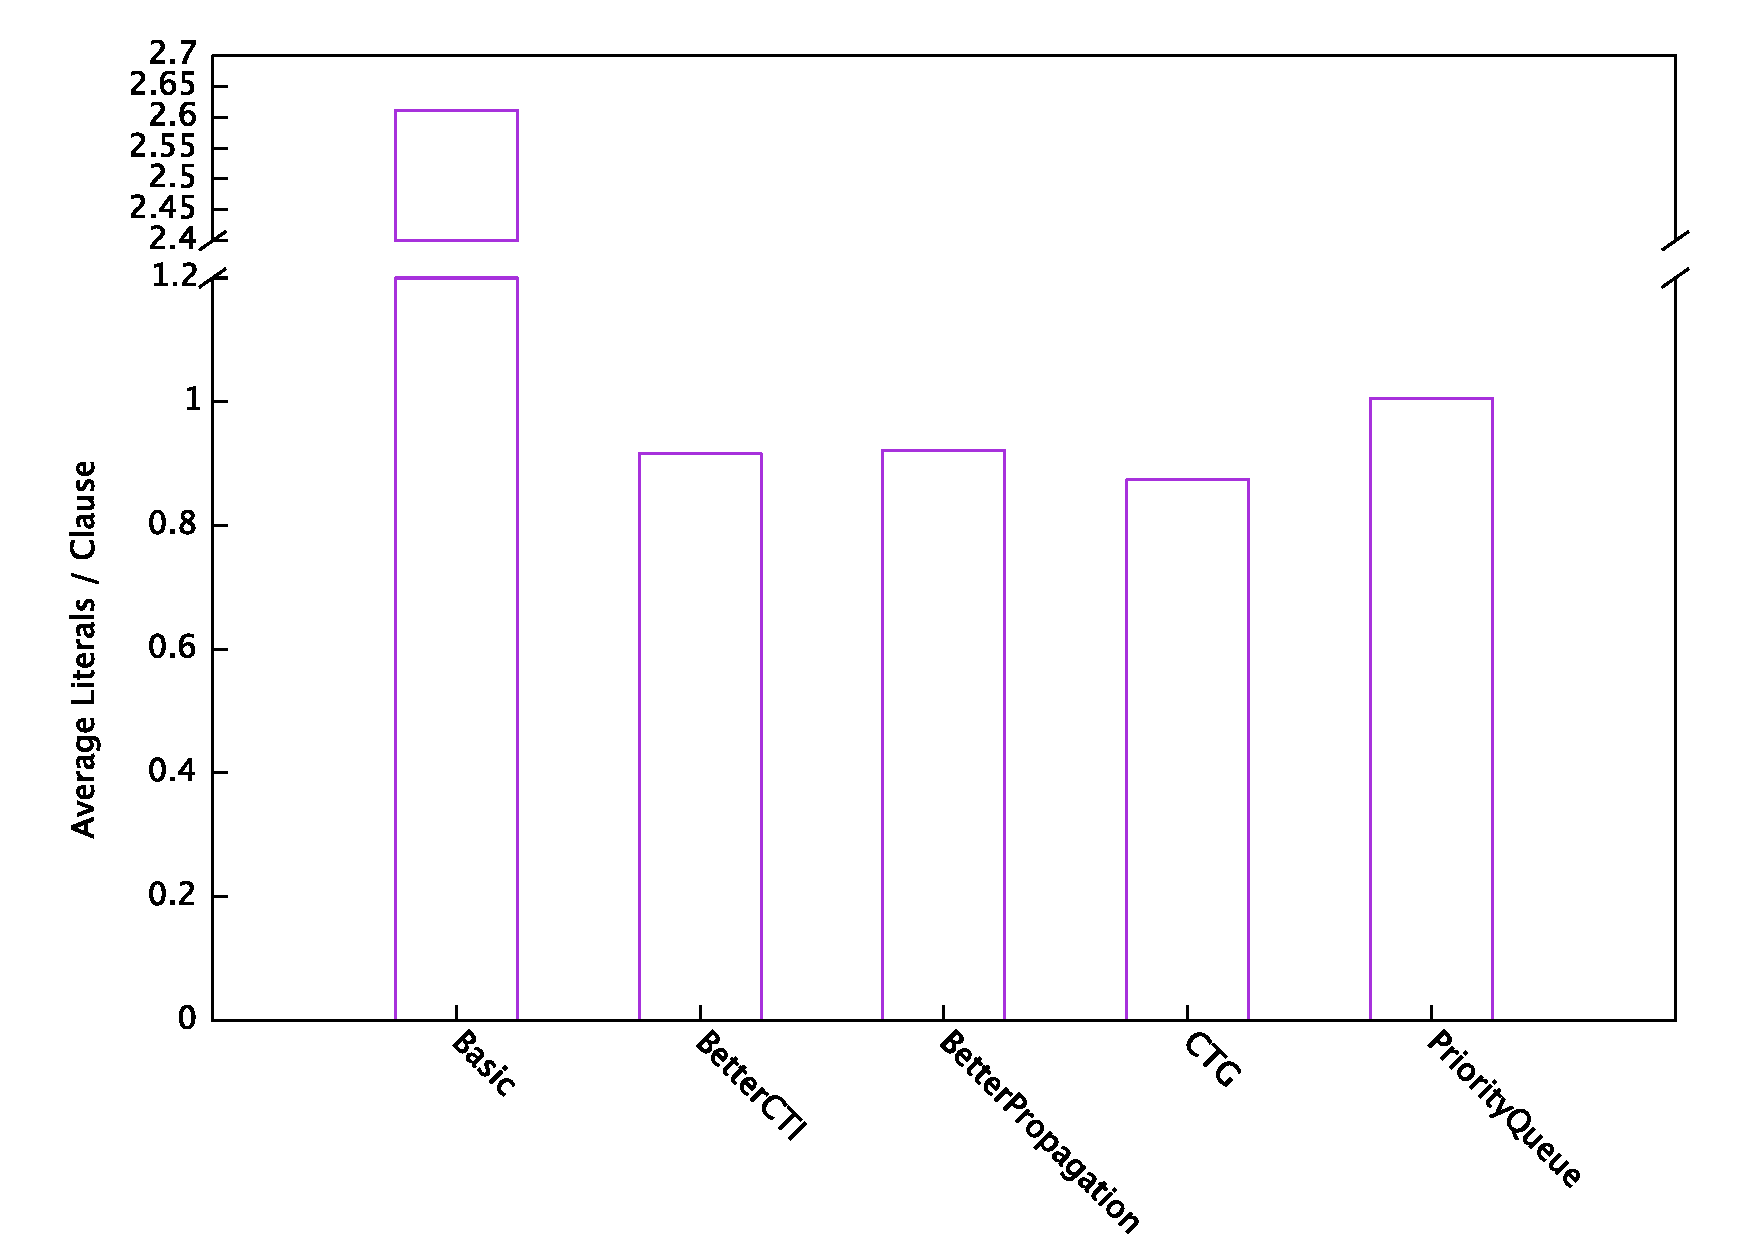
\includegraphics[width=16cm]{litspercls.pdf}
\caption{Average literals per clause averaged over the 14 handwritten examples and 50
 Hardware
Model Checking Competition examples.}
\label{eval:lits}
\end{figure}

\begin{figure}[t]
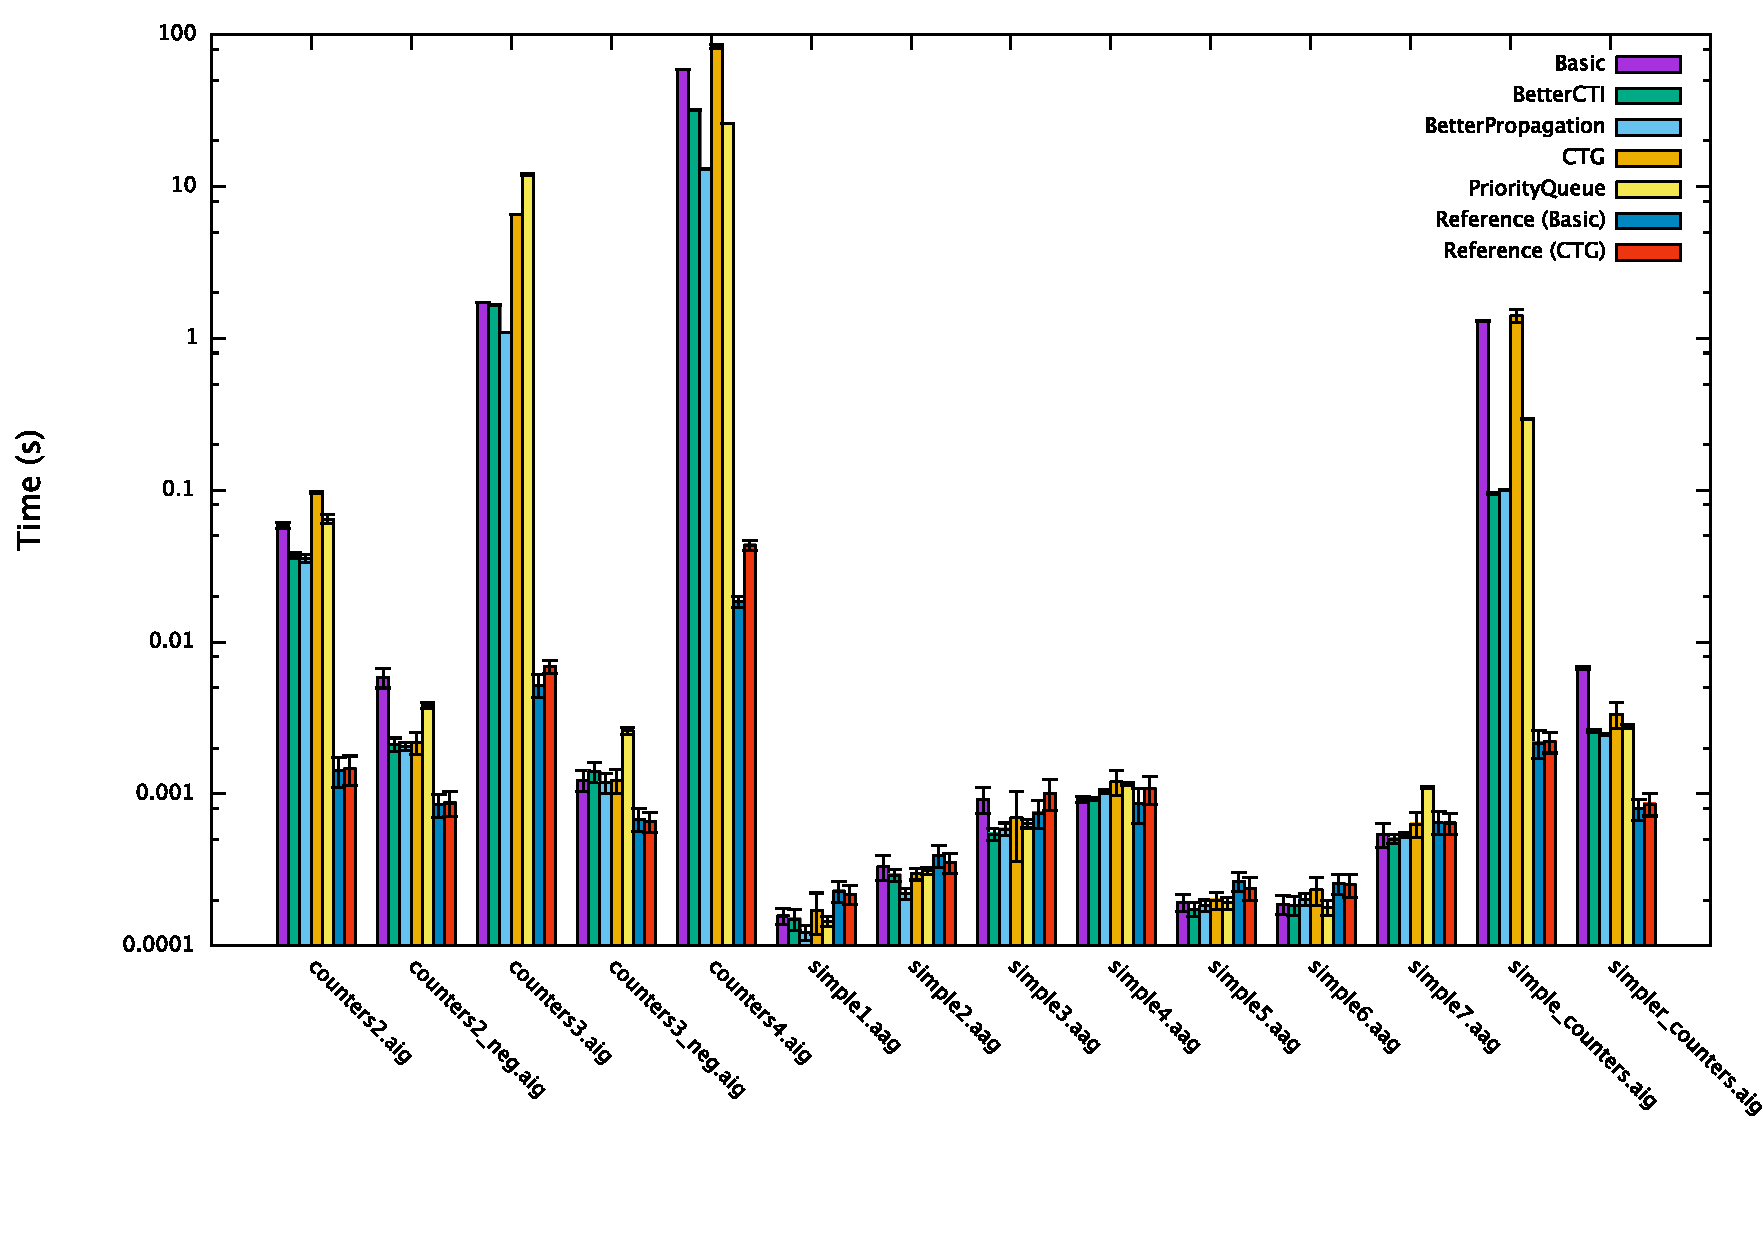
\includegraphics[width=16cm]{handwritten.pdf}
\caption{Benchmark results for the 14 handwritten examples on a log scale. Whiskers
indicate one standard deviation above and below the average time.}
\label{eval:time}
\end{figure}

\begin{figure}[!ht]
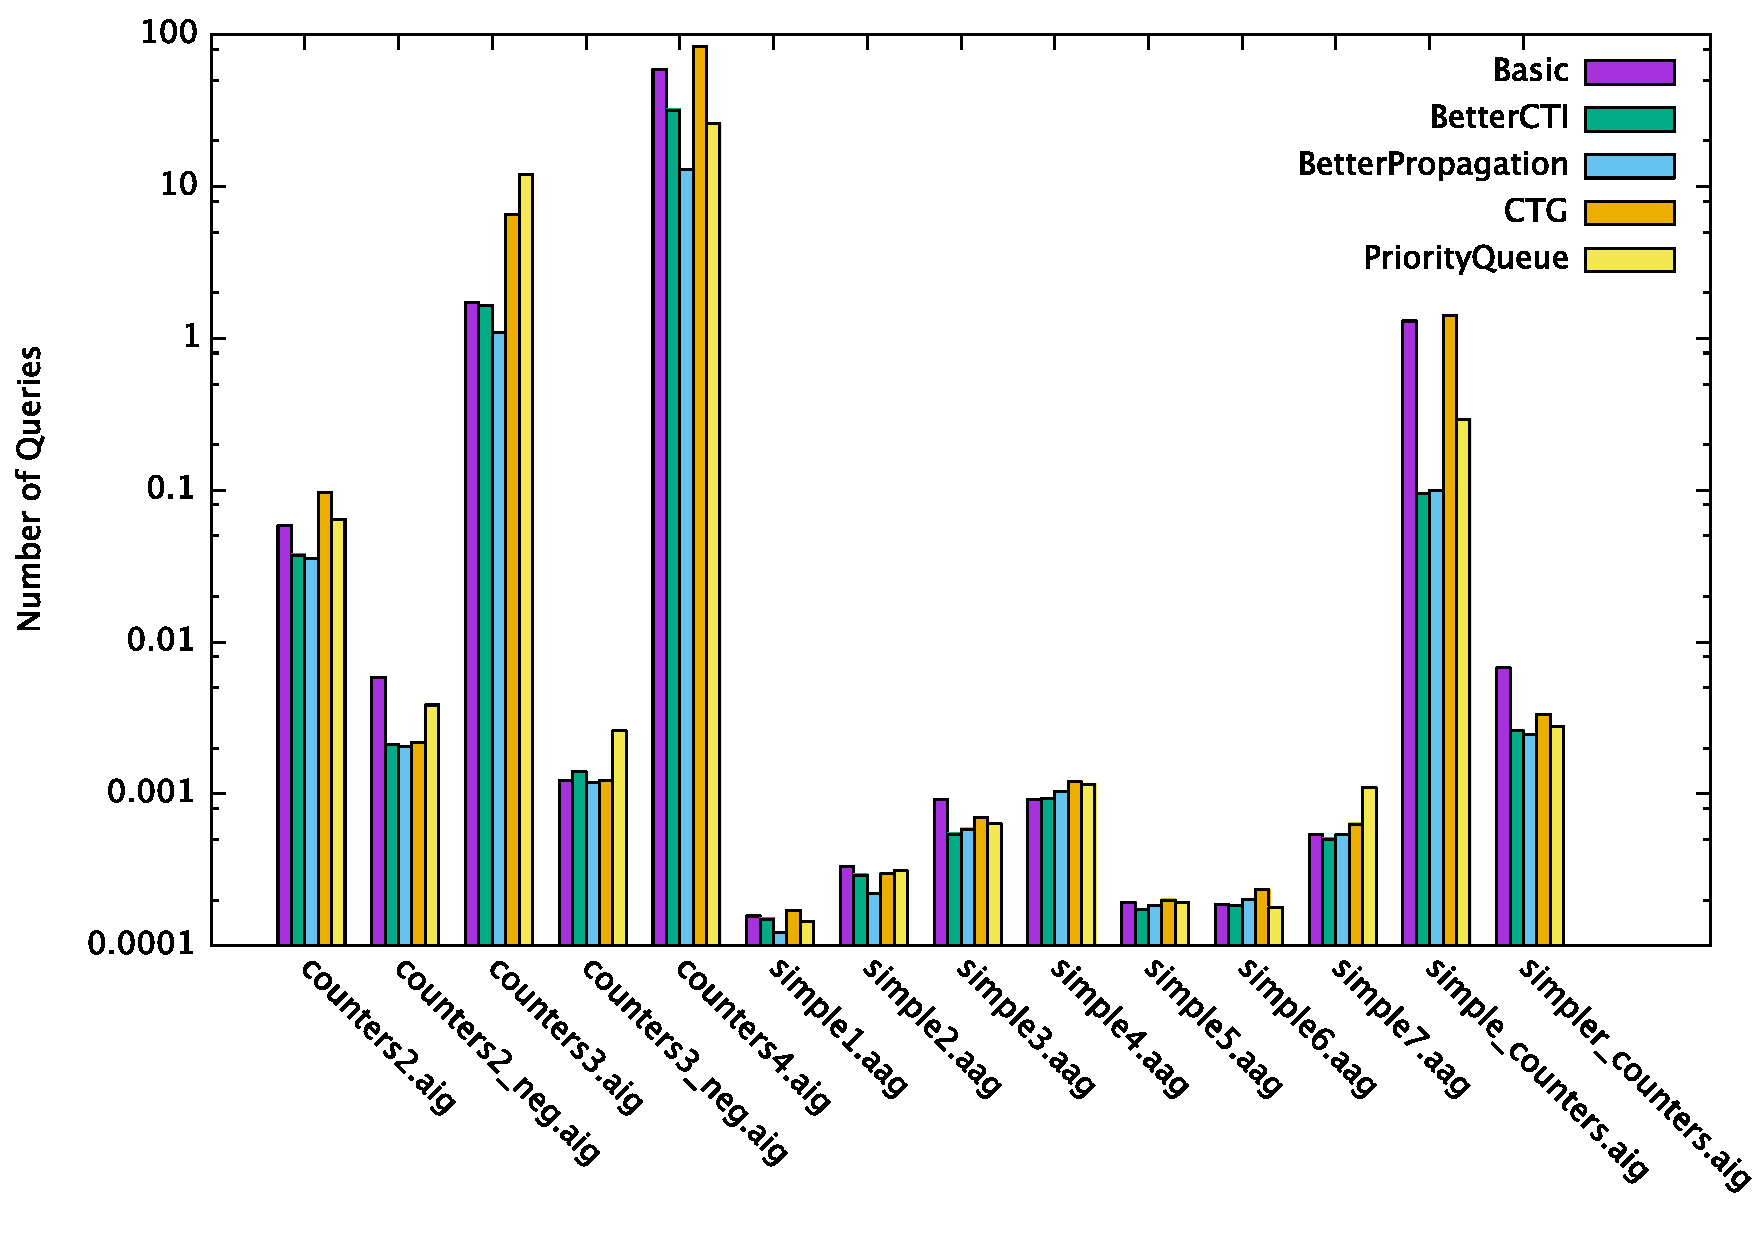
\includegraphics[width=16cm]{numqueries.pdf}
\caption{Number of queries for each variant run on the 14 handwritten examples on a log scale.}
\label{eval:queries}
\end{figure}

\paragraph{Smaller Counterexamples to Induction}{
The \emph{BetterCTI} implementation exhibits consistently
better performance than the \emph{Basic} implementation for examples
that require finding at least one CTI. In such cases,
discovering CTI clauses with fewer literals leads, as expected, to a smaller average number of
literals per clause (as seen in Figure \ref{eval:lits}), which suggests smaller SAT queries.

As mentioned previously, because the \emph{BetterCTI} implementation uses
CTIs that encompass sets of states rather than single states, when a negated CTI is proven at a depth
$k$, several states have been shown to be unreachable within $k$ steps of the transition relation
from the initial state. Dealing with a set of CTI states rather than a single CTI state
at a time allows
the \emph{BetterCTI} implementation to deal with fewer CTIs in some cases,
%(because the CTI sets of states
%may encompass several CTI states)
leading to fewer queries.
Benchmark results
agree with these expectations; for examples that require finding more than one CTI, \emph{BetterCTI}
finds fewer CTIs and makes fewer queries.
For example, the \emph{Basic} variant finds 59 CTIs and makes 414 queries to solve
\verb,shortp0.aig,, but the \emph{BetterCTI} variant only finds 3 CTIs and makes 49 queries, an order of magnitude improvement (see Appendix \ref{benchmarks}). 

The improvement of finding more general CTIs enabled the \emph{BetterCTI} variant of the implementation
(and all other implementations that include finding smaller CTIs) to
solve six more examples (\verb,counterp0.aig,, \verb,counterp0neg.aig,, \verb,pdtvishuffman7.aig,, 
\verb,pdtvismiim3.aig,, \verb,6s318r.aig,, \verb,srg5ptimo.aig,) than the \emph{Basic} version without
timing out.}

\paragraph{Propagation}{
Removing subsumed clauses (see Section \ref{impl:propagation}) also results in better performance on several
examples. While the performance impact that the improvement has is less drastic than the improvement of
\emph{BetterCTI} over \emph{Basic}, the \emph{BetterPropagation} version performs
considerably better
than the \emph{BetterCTI} version on the \verb,counters3.aig, and \verb,counters4.aig, examples in
particular (as seen in Figure \ref{eval:time}), where the adjustments allow the algorithm to prove the safety properties using fewer
queries (as seen in Figure \ref{eval:queries}). Even for examples such as \verb,pdtvismiim3.aig,, where \emph{BetterPropagation} makes more
queries than \emph{BetterCTI}, \emph{BetterPropagation} manages to perform better than \emph{BetterCTI}
because it makes smaller queries.}

\paragraph{Counterexamples to Generalization}{
The \emph{CTG} variation that deals with CTGs (see Section \ref{impl:generalization})
performs worse than the \emph{BetterPropagation} version
on examples, even in cases where \emph{CTG} reduces the average number of frames per clause (see Figures \ref{eval:time}, \ref{eval:lits}).
The most likely cause is that the examples used are too small for the performance benefit of
using CTGs to eliminate more states
to overcome the overhead of finding and proving negated CTGs;
finding and proving negated CTGs requires
making additional queries on each call to the \verb,inductiveGeneralization, function.

Similar results can be found
in the performance of \emph{IC3ref} with basic generalization and
improved (CTG-using) generalization on the same examples: for these small examples,
the reference implementation performs better overall with CTG-handling disabled.}

\paragraph{Priority Queues}{
The \emph{PriorityQueue} implementation generally does not perform as well as the
other variants, with the exception of \emph{CTG} (as seen in Figure \ref{eval:time}).
This result disagrees with findings that implementations of IC3 that
use priority queues are more efficient than simple recursive implementations
\cite{een11,griggio14}.

One of the performance advantages of the \emph{PriorityQueue} implementation is that CTIs do not need
to be rediscovered \cite{een11}: after a proof obligation $(s,i)$ is enqueued, until the algorithm fails or finds a fixed point,
the queue will always contain a proof obligation $(s,j)$ for $j \geq i$. When the proof obligation $(s,i)$
fulfilled at a certain depth $i$, $(s,i + 1)$ is enqueued.

Considering an example can help understand how re-enqueuing fulfilled obligations at
greater depths prevents the need to rediscover CTIs.
If $s$ is a CTI for proving a property
$p$ at depth $i + 2$, then the proof obligation $(s, i+1)$ must be fulfilled
in order to fulfill proof obligation $(\neg p, i+2)$. If $(s,i)$ is already
in the priority queue, \verb,proveObligations, must fulfill and
remove $(s,i)$ from the
priority queue and enqueue $(s, i + 1)$; it must then fulfill and remove $(s, i + 1)$ before
reaching proof obligation $(\neg p, i + 2)$. By the time \verb,proveObligations,
attempts to fulfill $(\neg p, i + 2)$, the CTI $s$ has already been proven
unreachable in $i + 1$ steps; if there is a CTI preventing a proof obligation
from being fulfilled after $(s,i)$ has been fulfilled, the CTI must be different
from $s$.

The \emph{PriorityQueue} implementation performs inductive generalization for each CTI only once, though,
when that CTI's first proof obligation is first enqueued. Rediscovering CTIs would allow the CTIs to
be generalized relative to later frames as well, rather than only to the first frame relative to which
the negated CTI is inductive. Not generalizing CTIs relative to later frames may
explain \emph{PriorityQueue}'s higher average number of
literals per clause (which suggests larger queries and worse performance).
}

\section{Reference Implementation}
\label{eval:ic3ref}
%Discuss performance comparison of final implementation with
%IC3 reference implementation, taking into account differences between
%the implementations.

The performance of the \emph{MC} variants is, for all except very small examples
(e.g. \verb,simple1.aag,),
worse compared to the performance of \emph{IC3ref}
with or without generalization involving CTGs enabled (as seen in Figure \ref{eval:time}).

The choice of implementation language may account for much of the difference in performance, as the reference
implementation in C++ has more control over memory allocations than the implementations in Haskell, which is
a garbage-collected language. I mention other differences between the implementations that may explain
some of the performance differences below.

\subsubsection{Model Representation}
\label{eval:ic3ref:model}
The reference implementation represents hardware models differently from
\emph{MC}, which may account for some of the performance differences.
The reference implementation keeps track of which variables are inputs, latches, and AND gates.
Each \emph{IC3ref} \verb,Model, maintains both the primed and current values for inputs and latches and keeps a
table to memoize the values of AND gates.

As mentioned earlier, when the consecution query $F_k \wedge T \Rightarrow P'$ fails, this corresponds
to the CNF query $F_k \wedge T \wedge \neg P'$ being satisfiable.
While a full satisfying assignment
$s$ gives a CTI state, it is better to use a set of states $c \subset s$ as a CTI cube, so that several
CTI states can be eliminated at once.
The \verb,stateOf, function uses the information kept in \verb,Model,s to extract the smaller
cube from the model $s$ giving the satisfying assignment for a failed consecution query directly,
without further SAT-solver queries.

The \emph{MC} variants implement the IC3 algorithm more directly and do not store as
much information in their hardware
models. They instead use several SAT-solver queries to extract the necessary literals
from $s$.

\subsubsection{MiniSat}
\label{eval:ic3ref:minisat}
The reference implementation is more closely coupled to MiniSat's implementation. Because both the reference
implementation and MiniSat are written in C++, the reference implementation can and does call MiniSat functions
and instantiate MiniSat objects (e.g. \verb,SimpSolver,s) directly.
In contrast, the Haskell implementations
must interact with MiniSat through an interface and suffer from associated overheads, such as those from
marshalling data from the data structures returned from the C wrapper for MiniSat into the corresponding
Haskell data structures.

The reference implementation also makes use of empirical results to improve the performance of MiniSat queries.
For example, in the \verb,stateOf, function, which extracts a model from a failed consecution query
(to e.g. find a CTI cube), the set of literals passed to the MiniSat \verb,Solver, are reordered according
found to be the best choice empirically \cite{minisat}.

\subsubsection{Overall Structure}

The reference implementation is implemented in an imperative language and
uses a priority queue, resulting in a different structure from the
\emph{MC} implementations. It also handles proof obligations
differently than the \emph{PriorityQueue} implementation does.
The \emph{PriorityQueue} implementation tries to improve performance by
preventing the rediscovery of
CTIs and reducing the number of generalization attempts,
but \emph{IC3ref} does not.

For a CTI $s$ that prevents the fulfillment
of a proof obligation at depth $i$, the reference implementation enqueues proof
obligation $(s,i - 1)$
and performs generalization relative to the frame $F_{i - 1}$ each time $\neg s$ has been shown
to be inductive relative to frame $F_{i - 1}$. Generalization does not seem
to be as expensive for \emph{IC3ref} as \emph{MC}, probably as a
result of the model representation (Section \ref{eval:ic3ref:model}) and
MiniSat interface (Section \ref{eval:ic3ref:minisat}) differences.

Because the reference implementation does not prevent CTIs from being rediscovered,
it does not
enqueue a new proof obligation $(s, i+1)$ each time a proof obligation $(s, i)$ has been
fulfilled, unlike \emph{PriorityQueue}.
The efficiency of \emph{IC3ref}'s other components compensates
for the performance disadvantage of needing to rediscover CTIs.
The safety property is maintained and
handled separately from CTIs; its negation is not included as part of a proof obligation
placed in the priority queue.

\chapter{Conclusion}
\label{conc}

This chapter summarizes the work done and goals met for this project and gives
suggestions for further extensions to the project.

The IC3 algorithm provides a new way to perform SAT-based symbolic model checking of
safety properties of hardware, and the performance of its initial implementation
\verb,ic3, in HWMCC'10 resulted in the development of several variants of
and extensions to the algorithm.

This project's main goal is to implement a model checker that uses the IC3 algorithm.
This goal was achieved by meeting the success criteria outlined in
the project proposal:

\begin{itemize}
\item I met the requirement that an AIGER parser must be implemented by understanding
the AIGER format (Section \ref{prep:aiger}) and writing the parser (Section
\ref{impl:aiger}).
\item I met the requirement that a MiniSat interface must be implemented by
learning about MiniSat (Section \ref{prep:minisat}) and writing a Haskell
interface to it (Section \ref{impl:minisat}).
\item I met the requirement that a basic version of the IC3 algorithm must be
implemented by
understanding the IC3 algorithm (Section \ref{prep:ic3}) and implementing the
\emph{Basic} variant (Section \ref{impl:modelchecker}).
\item I verified that the requirement that the model checker correctly solves some small
examples through testing and validating against \emph{IC3ref}
(Section \ref{eval:solving}).
\end{itemize}

The project aims and success criteria were exceeded with the implementation of other
IC3 back ends for \emph{MC} (Section \ref{prep:ic3})
and the ability of \emph{MC} to correctly check examples
from the HWMCC (Section \ref{eval:solving}).

%\section{Project Details}
In the process of completing the project, I have written code and hardware model
examples, the quantity of which is captured in the following table:
\begin{center}
\begin{tabular}{| l | l |}
\hline
Language & Lines of Code\\
\hline
Haskell (\emph{Basic} variant) & 946\\
C++ & 70\\
C/C++ header & 44\\
AIGER & 65\\
BLIF & 233\\
\hline
\end{tabular}
\end{center}

The code for this project may be found at \url{https://github.com/lmp47/ModelChecker}.

\paragraph{Further Work}{
Instead of the extensions mentioned in the initial project proposal,
I elected to implement other variants of the model checker and examine their
effects on the model checker's performance.
As a result, interfacing with different SAT solvers and implementing lazy
abstraction-refinement remain as future work.

Implementing interfaces with different SAT solvers may allow more examples to be solved efficiently.
Aaron Bradley notes that the performance of the IC3 algorithm is considerably affected
by the behavior of the SAT solver it uses \cite{bradley12}; even if each SAT query takes the same amount of
time, the algorithm's performance may still vary if the SAT solver behaves even slightly differently.
Because the choice of SAT solver may affect which examples can be solved efficiently, allowing the model
checker to use different SAT solvers may increase the number of examples that can be solved.

Abstraction-refinement is a technique used in verification to mitigate the effects
of the state explosion problem. Abstraction removes irrelevant details of the model,
and if the abstraction is found to be too coarse at some point during verification,
refinement can add necessary details of the model back into the abstraction.
Yakir Vizel, Orna Grumberg, and Sharon Shoham introduced a abstraction-refinement
scheme that is compatible with the IC3 algorithm \cite{vizel12}. The implementation
of this modified algorithm achieved significant speedups compared with the
original IC3 algorithm implementation \verb,ic3,, and a variant
of the model checker in Haskell that uses this abstraction-refinement scheme may 
exhibit a similar improvement.}
%The modified algorithm uses different
%abstractions for the different approximated sets of states (i.e. frames). Upon

%%%%%%%%%%%%%%%%%%%%%%%%%%%%%%%%%%%%%%%%%%%%%%%%%%%%%%%%%%%%%%%%%%%%%
% the bibliography
\addcontentsline{toc}{chapter}{Bibliography}
\bibliography{refs}

%%%%%%%%%%%%%%%%%%%%%%%%%%%%%%%%%%%%%%%%%%%%%%%%%%%%%%%%%%%%%%%%%%%%%
% the appendices
\appendix

\chapter{AIGER Format}
\label{aiger}
This appendix describes the binary version of the old AIGER format
and the new version of the AIGER format by
comparison with the old format.

\paragraph{Binary version}{
The binary version assumes that variable indices always
occur in increasing order. Each literal must be defined, so this assumption
allows some indices to be omitted when defining components.
Inputs are not explicitly listed; input variables are inferred based on
the value of \verb,I,.
Latches are specified by only listing next-state
indices, and AND gates are represented by two differences (that tend to be
small in practice).
%These assumptions allow AND gates to be represented by two differences
%that tend to be small in practice.

The binary format assumes that inputs to an AND gate
have been defined before the gate.
For an AND gate specified in the ASCII format by \verb,lhs rhs0 rhs1,,
where inputs \verb,rhs0, and \verb,rhs1, are ordered such that
$\verb,rhs0, \geq \verb,rhs1,$, define
$\delta_0 = \verb,lhs, - \verb,rhs0,$
and
$\delta_1 = \verb,lhs, - \verb,rhs1,$.
For 7-bit words $w_0, \ldots w_n$ with
$\delta_i = w_0 + 2^7w_1 + \ldots + 2^{7n}w_n$,
$\delta_i$ is represented as the sequence of $n + 1$ bytes
$b_0, \ldots, b_n$.
For $0 \leq k < n$, $b_k$ is the byte obtained by setting the most
significant bit to 1 and the other bits to $w_k$. The byte
$b_n$ is obtained by setting the most
significant bit to 0 and the rest of the bits to $w_n$.
This binary encoding gives a more compact representation for AND
gates than the ASCII format.
}

\paragraph{New version} {
The new format appends new counts \verb,B C J F, to the old
format header.
%\begin{verbatim}
%V M I L O A B C J F
%\end{verbatim}
%where \verb,V,, \verb,M,, \verb,I,, \verb,L,, \verb,O,, \verb,A, are as
%in the old format.
\verb,B, gives the number of ``bad state'' properties,
\verb,C, gives the number of invariant constraints,
\verb,J, gives the number of justice properties, and
\verb,F, gives the number of fairness constraints.
The header can be truncated
after the AND-gate count if all remaining counts are
zero, making the new format
backward compatible.

The ``bad state'' properties allow negated safety properties to be specified
separately from outputs.
The invariant constraints allow for the specification of properties that
hold at all states up to and including the state where the ``bad state''
holds.
Justice and fairness constraints are not used by
\emph{MC} and will not be explained further.

Components are specified after the header in the same order that their
counts occur in the header with the exception of AND gates, which
occur last. Latches' initial values can now be specified
with an additional index after the next-state index.
This index can be \verb,0,, \verb,1,, or the index of the latch itself,
in which case the latch is uninitialized.
If the initial value is omitted, the initial value is assumed to be
0, as in the old version of the format.
The new version of the format is otherwise
the same as the old format.}

\chapter{Code Extracts}
%This appendix contains some code extracts from the project implementation.

\begin{figure}[H]
\centering
\begin{lstlisting}
inductiveGeneralization :: Clause -> Frame -> Frame -> Model -> Word -> Clause
inductiveGeneralization clause f0 fk m = generalize clause f0 fk []
  where
    generalize cs _ _ needed 0 = cs ++ needed
    generalize [] _ _ needed _ = needed
    generalize (c:cs) f0 fk needed k = 
      let res = solveWithAssumps
                  (solver (getFrameWith ((cs ++ needed):clauses fk) m))
                  (map (prime.neg) (cs ++ needed))
        if not (satisfiable res) && initiation f0 cs
          then generalize cs f0 fk needed k
          else generalize cs f0 fk (c:needed) ( k - 1 ) 
\end{lstlisting}
\caption{The function that approximates the {\it mic} algorithm in the most basic way.}
\label{inductiveGeneralization}
\end{figure}

\begin{figure}[H]
\begin{lstlisting}
parseTest :: String -> IO [Test]
parseTest name =
  do aigModel  <- Parser.getModelFromFile ("examples/" ++ name)
     aigModel' <- Tools.getModelFromFile ("examples/" ++ name)
     return (map TestCase
              [ assertEqual (name ++ " numVars") (numVars aigModel)
                            (numVars aigModel')
              , assertEqual (name ++ " numInputs") (numInputs aigModel)
                            (numInputs aigModel')
              , assertEqual (name ++ " latches") (sort (latches aigModel))
                            (sort (latches aigModel'))
              , assertEqual (name ++ " outputs") (sort (outputs aigModel))
                            (sort (outputs aigModel'))
              , assertEqual (name ++ " ands") (sort (ands aigModel))
                            (sort (ands aigModel')) ])
\end{lstlisting}
\caption{The function for testing the AIGER parser on files in the {\tt examples} directory.}
\label{parseTest}
\end{figure}

\chapter{Benchmark Results}
\label{benchmarks}

In the following tables, ``Average Literals per Clause'' is abbreviated as
``ALC,'' and ``Standard Deviation'' is abbreviated as ``SD.''

\section{Basic}
\csvreader[longtable=|l|p{3em}|p{3.5em}|l|l|p{4.5em}|p{4em}|,
    table head= \hline Name & Frames & ALC & CTIs & Queries & Mean Time (s) & SD of
Time(s)\\\hline,
    late after line=\\\hline]%
{basic.csv}{name = \name, frames = \frames, litspercls = \litspercls, ctis = \ctis, queries = \queries, time = \time, stdev = \stdev}%
{\name & \frames & \litspercls & \ctis & \queries & \time & \stdev}%

\section{BetterCTI}
\csvreader[longtable=|l|p{3em}|p{3.5em}|l|l|p{4.5em}|p{4em}|,
    table head= \hline Name & Frames & ALC & CTIs & Queries & Mean Time (s) & SD of Time
(s)\\\hline,
    late after line=\\\hline]%
{betterCTI.csv}{name = \name, frames = \frames, litspercls = \litspercls, ctis = \ctis, queries = \queries, time = \time, stdev = \stdev}%
{\name & \frames & \litspercls & \ctis & \queries & \time & \stdev}%

\section{BetterPropagation}
\csvreader[longtable=|l|p{3em}|p{3.5em}|l|l|p{4.5em}|p{4em}|,
    table head= \hline Name & Frames & ALC & CTIs & Queries & Mean Time (s) & SD of Time
(s)\\\hline,
    late after line=\\\hline]%
{betterPropagation.csv}{name = \name, frames = \frames, litspercls = \litspercls, ctis = \ctis, queries = \queries, time = \time, stdev = \stdev}%
{\name & \frames & \litspercls & \ctis & \queries & \time & \stdev}%

\section{PriorityQueue}
\csvreader[longtable=|l|p{3em}|p{3.5em}|l|l|p{4.5em}|p{4em}|,
    table head= \hline Name & Frames & ALC & CTIs & Queries & Mean Time (s) & SD of Time
(s)\\\hline,
    late after line=\\\hline]%
{priorityQueue.csv}{name = \name, frames = \frames, litspercls = \litspercls, ctis = \ctis, queries = \queries, time = \time, stdev = \stdev}%
{\name & \frames & \litspercls & \ctis & \queries & \time & \stdev}%

\section{CTG}
\csvreader[longtable=|l|p{3em}|p{3.5em}|l|l|l|p{4.5em}|p{4em}|,
    table head= \hline Name & Frames & ALC & CTIs & CTGs & Queries & Mean Time (s) & SD of Time (s)\\\hline,
    late after line=\\\hline]%
{ctg.csv}{name = \name, frames = \frames, litspercls = \litspercls, ctis = \ctis, ctgs = \ctgs, queries = \queries, time = \time, stdev = \stdev}%
{\name & \frames & \litspercls & \ctis & \ctgs & \queries & \time & \stdev}%

%\section{Reference Implementation}

\chapter{Project Proposal}

% A project proposal.
% The format draws heavily on the example project proposal
% and the Model Project Proposals (and their LaTeX sources) available
% http://www.cl.cam.ac.uk/teaching/projects/

\documentclass[12pt,a4paper,twoside]{article}
\usepackage[pdfborder={0 0 0}]{hyperref}
\usepackage[margin=25mm]{geometry}
\usepackage{graphicx}
\begin{document}

\section*{Introduction and Description of the Work}
Model checking is one way of assessing whether or not a hardware or
software system has certain properties. For example, model checkers can be
used to check systems for safety properties by finding examples of states
that violate the properties or by proving that all states have the
properties.

Explicit-state model checking can be infeasible for systems with a large
number of states, but symbolic model checking, which represents
states and the transition relation between them as boolean expressions,
can handle more states. Symbolic model checking initially relied on the
efficient representation of boolean expressions through binary decision
diagrams (BDDs), but BDDs can still consume a large amount of space, and
finding an ordering for BDD variables that keeps the BDDs small can become
costly \cite{biere99}.

Symbolic model checking techniques that rely on SAT solvers provide an
alternative to BDD-based approaches. SAT-based approaches include
bounded model checking \cite{biere99} and $k$-induction \cite{demoura03},
but both of these approaches involve unrolling the transition relation,
which can lead to long SAT solver queries.

IC3 \cite{bradley11} is a more recently developed SAT-based algorithm for
the symbolic model checking of safety properties. Instead of unrolling the
transition relation and considering entire paths, IC3 maintains a set of
frames $F_0,...,F_k$, where each frame $F_i$ is an overapproximation of
the set of states reachable in at most $i$ steps, and considers at most one
step of the transition relation from a particular frame at a time.
As a result, IC3 can find inductive strengthenings that tend
to be smaller and more convenient than those found by BMC-based
techniques such as $k$-induction, which finds strengthenings that are the
negations of spurious counterexample paths \cite{demoura03}, and the SAT
queries that IC3 makes tend to be simpler \cite{bradley12}.

This project focuses on implementing a symbolic model checker for verifying
safety properties of hardware. The model checker will include a new
implementation of the IC3 algorithm in Haskell, which will make use of an
existing SAT solver.

\section*{Starting Point}

I begin the project with some experience programming in Haskell
from a summer internship and no experience with model checking or using
a SAT solver. I have informally acquired some knowledge about model checking
to formulate this project idea.

\section*{Substance and Structure of the Project}

The project aims to implement a hardware model checker that takes its
inputs in AIGER format and queries the MiniSat SAT solver.

\noindent The structure of the project can be broken down into the following
components:

\begin{enumerate}

\item {\bf Parsing AIGER format} The model checker takes its inputs in AIGER
format and will, as a result, require an AIGER parser. The AIGER format
is fairly simple and hand-coding a parser for it should be suitable.

\item {\bf Interfacing with MiniSat} The model checker
will be using the MiniSat SAT solver, so an API that allows the
model checker to query MiniSat will be required.

\item {\bf Implementing the IC3 algorithm} 
The main aspect of the project is the implementation of the IC3 algorithm.
The implementation will largely be based on the algorithm as described in
\cite{bradley11,bradley12}. 

\item {\bf Evaluating the model checker}
The model checker will be evaluated by measuring its performance on
checking examples. Though the project does not focus greatly on the
efficiency of the implementation, it may still be interesting to
see how the performance of this IC3 implementation in Haskell compares with
other implementations. As a result, benchmarks taken for the
model checker will be compared with further benchmarks taken for
Aaron Bradley's reference IC3 implementation, which is
implemented in C++.
Given that the reference implementation takes its inputs in AIGER format
and also uses MiniSat, the benchmarks should provide a means to compare
the IC3 implementations specifically.

\item {\bf Writing the dissertation}

\end{enumerate}

\subsection*{Possible Extensions}
If the aforementioned aspects of the project are completed, carrying out
the following extensions could be possible:
\begin{itemize}
\item Interfacing with other SAT solvers, and possibly performing additional
benchmarking; comparing the performance of the model checker when used with
different SAT solvers may be of interest since the performance
of IC3 implementations tend to vary considerably depending on the
characteristics of the underlying SAT solver.
\item Model checking properties of real hardware as a case study.
\item Implementing abstraction-refinement as described in \cite{vizel12}.
\end{itemize}


\section*{Success Criteria}

The project will be a success if the following have been completed:
\begin{itemize}
\item The AIGER parser has been implemented.
\item The MiniSat interface has been implemented.
\item The IC3 algorithm has been implemented.
\item The model checker should be able to solve some small examples.
\end{itemize}


\section*{Timetable: Workplan and Milestones}

\begin{enumerate}

\item {\bf 16 October 2015 -- 28 October 2015}

Preliminary reading. Get familiar with the AIGER format, MiniSat and
relevant Haskell libraries and tools for implementing the components
of the project.

\item {\bf 29 October 2015 -- 4 November 2015}

Write an AIGER format parser.
\\
Milestone: Parser completed. Relevant information from
AIGER files can be extracted.

\item {\bf 5 November 2015 -- 18 November 2015}

Implement a MiniSat interface.
\\
Milestone: MiniSat interface completed, enabling the model checker to use
MiniSat to solve SAT problems.

\item {\bf 19 November 2015}

Begin implementing the IC3 algorithm.

\item {\bf Michaelmas vacation}

Continue implementing the IC3 algorithm.

\item {\bf 14 January 2016 -- 27 January 2016}

Write progress report. Finish implementation of the IC3 algorithm.
\\
Milestones: Progress report completed.
Working implementation of the model checker completed.

\item {\bf 28 January 2016 -- 10 February 2016}

Measure and compare this IC3 implementation's performance and the reference
implementation's performance.
\\
Milestone: Evaluation completed.

\item {\bf 11 February 2016 -- 11 March 2016}

Write the main parts of the dissertation.
\\
Milestone:
Finished writing main parts of dissertation: introduction, preparation,
implementation and evaluation chapters.

\item {\bf Easter vacation}

If necessary, use this time for catching up.
Otherwise, work on extensions, starting with interfacing with other
SAT solvers.
Finish writing dissertation.
\\
Milestones: All implementation and evaluation completed.
Draft dissertation completed.

\item {\bf 21 April 2016 -- 4 May 2016}

Proofread and edit dissertation as necessary.
\\
Milestone: Dissertation ready for submission.

\item {\bf 5 May 2016 -- 13 May 2016}

Time left for catching up in case any delays have occurred in the
completion of any milestones.
\\
Milestone: Dissertation submitted.

\end{enumerate}

\section*{Resources Required}

For the project I will mostly make use of my laptop, which runs OS X 10.8.
I accept full responsibility for this machine and I have made contingency
plans to protect myself against hardware and/or software failure. 
If my main computer fails, I will use MCS computers.
I will use GitHub for backup and git for revision control.

\noindent I will also be using:
\begin{itemize}
\item AIGER utilities, available \url{http://fmv.jku.at/aiger/}
\item MiniSat, available \url{https://github.com/niklasso/minisat}
\item Models from the Hardware Model Checking Competition, such as those
available \url{http://fmv.jku.at/hwmcc10/}
\item Aaron Bradley's Reference IC3 implementation, available
\url{https://github.com/arbrad/IC3ref}
\end{itemize}
\end{document}


\end{document}

